\documentclass[conference]{IEEEtran}
\IEEEoverridecommandlockouts
\usepackage{cite}
\usepackage{amsmath,amssymb,amsfonts}
\usepackage{soul}
\usepackage{pifont}
\usepackage{siunitx}
\sisetup{group-separator = {,}, group-minimum-digits = 4}
\usepackage{threeparttable}
\usepackage{tabularx}
\usepackage{tikz}
\usepackage{multirow}
\usepackage{pgfplots}
\pgfplotsset{compat=1.18}  
\usepackage{pgfplotstable}
\usepackage{booktabs,array}
\usepackage{algorithmic}
\usepackage{graphicx}
\usepackage{textcomp}
\usepackage{xcolor}
 %dari ko nag start add sa package
\usepackage{ragged2e}
\usepackage{multirow}
\usepackage{array}
\usepackage{hyperref}
\usepackage{pgf-pie}

\def\BibTeX{{\rm B\kern-.05em{\sc i\kern-.025em b}\kern-.08em
    T\kern-.1667em\lower.7ex\hbox{E}\kern-.125emX}}
\begin{document}

\title{Enhanced Black Sigatoka Detection Using Multi-Stage Wiener-Wavelet-Median Filtering with Wavelet and Fourier Transform Features}

%Authors
\author{
	\IEEEauthorblockN{Mark Madorable}
	\IEEEauthorblockA{
    \textit{Computer Engineering Department} \\
    \textit{University of Science and Technology} \\
    \textit{of Southern Philippines}\\ 
    Cagayan de Oro City, Philippines \\
    mark.madorable@2.ustp.edu.ph}
	\and
    \IEEEauthorblockN{Mary Ann Calalin}
	\IEEEauthorblockA{
	\textit{Computer Engineering Department} \\
	\textit{University of Science and Technology} \\
	\textit{of Southern Philippines}\\ 
	Cagayan de Oro City, Philippines \\
	maryann.calalin@2.ustp.edu.ph}
	\and
	\IEEEauthorblockN{Aljhon Mangmang}
	\IEEEauthorblockA{
    \textit{Computer Engineering Department} \\
    \textit{University of Science and Technology}  \\
    \textit{of Southern Philippines}\\ 
    Cagayan de Oro City, Philippines \\
    aljhon.mangmang@2.ustp.edu.ph}
}

\maketitle

\begin{abstract}
\hl{This document is a model and instructions for \LaTeX.
This and the IEEEtran.cls file define the components of your paper [title, text, heads, etc.]. *CRITICAL: Do Not Use Symbols, Special Characters, Footnotes, 
or Math in Paper Title or Abstract.}
\end{abstract}

\begin{IEEEkeywords}
component, formatting, style, styling, insert
\end{IEEEkeywords}

\section{Introduction}
\label{introduction}

Bananas (\emph{Musa} spp.) represent one of the most vital tropical fruit crops globally and serve as a cornerstone of the Philippine agricultural economy \cite{evans2020banana}. In 2023, the Philippines produced approximately 7.9 million metric tons, ranking as the fifth largest producer worldwide \cite{voora2023global}. Moreover, Northern Mindanao follows the Davao Region as the second-largest producer \cite{PSABanana2023}, underscoring the crop’s economic importance in the region. 

However, the Philippine banana industry faces persistent threats from diseases, particularly Black Sigatoka (Black Leaf Streak) caused by the ascomycete fungus \emph{Pseudocercospora fijiensis}, which can reduce yields by up to 50\% \cite{jomanga2021effects}.

Traditional detection methods for Black Sigatoka, such as manual field inspections, are time-consuming and subjective \cite{escudero2021development}, while laboratory-based techniques like Polymerase Chain Reaction (PCR) are costly and impractical for large-scale monitoring \cite{da2025resistance}. Recent studies using computer vision and machine learning have shown promise, with Chaudhari and Patil \cite{chaudhari2020banana} achieving $85\%$ accuracy using Gray Level Cooccurrence Matrix (GLCM) for texture feature extraction and mean, kurtosis and skewness for color feature extraction. Another study, by Escudero, et al. \cite{escudero2021development}, achieved $80.58\%$ accuracy in detecting Black Sigatoka severity using wavelet and Fourier features combined with ensemble classifiers. Further, the study of Evuri \cite{evuri2023banana} attained a high $90\%$ accuracy using GLCM and Neighbouring Grey Tone Difference Matrix (NGTDM) for feature extraction and image sharpening method.

Although these mentioned studies demonstrate progress in Black Sigatoka disease detection, they share important gaps that limit practical deployment. Evuri \cite{evuri2023banana} focused on Support Vector Machine (SVM) with GLCM and NGTDM features and achieved high accuracy, but the experiment used a small, imbalanced, laboratory-controlled dataset, relied only on two diseases, and did not test performance under real field conditions such as lighting variability, noise, or complex backgrounds. In addition, Escudero, et al. \cite{escudero2021development} addressed real-world constraints more directly by creating a mobile support system with a custom dataset and validating it with farmers, yet their model achieved only $80.58\%$ efficiency, with no inclusion of noise reduction methods. Meanwhile, the multi-feature SVM study by Evuri and comparable works emphasize handcrafted features but lack robust preprocessing and noise-reduction strategies which are essential when dealing with field images containing shadows, blur, and uneven illumination. Across all reviewed studies, early-stage detection remains difficult, datasets are restricted in diversity and class coverage, and no work integrates a comprehensive noise-removal pipeline or evaluates model robustness under the wide visual variation typical of agricultural environments.

Hence, this study addresses these limitations by proposing an enhanced computer vision system for Black Sigatoka detection that integrates advanced noise reduction techniques with optimized feature extraction. The main contributions include:

\begin{enumerate}
\item A multi-stage image pre-processing pipeline incorporating Wiener filtering, median filtering, and wavelet-based denoising for improved performance under variable field conditions
\item An optimized feature extraction framework combining color, texture, and spectral features
\item Enhanced segmentation and classification methods specifically designed for  detection and,
\item Comprehensive evaluation demonstrating improved robustness and accuracy compared to existing approaches
\end{enumerate}

The remainder of this paper is organized as follows: Section II reviews related work in plant disease detection. Section III details our methodology. Section IV presents experimental results and discussion. Section V concludes with findings and future research directions.  

\section{Literature Review}
\label{literaturereview}
\subsection{Etiology and Economic Impact of Black Sigatoka}
Bananas are a vital crop in the Philippines, a top global producer where cultivation is concentrated in regions like Davao and Northern Mindanao (Figs. \ref{fig:banana_global}, \ref{fig:banana-production}) \cite{evans2020banana, voora2023global, PSABanana2023}. This economic importance is threatened by Black Sigatoka, a devastating fungal disease. The infection progresses from dark leaf streaks (Fig. \ref{fig:symptom_progression}a) to necrotic lesions (Fig. \ref{fig:symptom_progression}b) and ultimately extensive leaf death (Figs. \ref{fig:symptom_progression}c, \ref{fig:symptom_progression}d), which severely compromises the plant's photosynthetic capacity \cite{george2022symptomatology, nelson2008black}.

The economic impact of Black Sigatoka is twofold. By destroying leaf area, the disease can suppress fruit yields by up to 50\% \cite{jomanga2021effects}. To prevent such catastrophic losses, producers are forced into a costly regime of frequent fungicide applications. This combination of significant revenue loss and heightened production costs creates a persistent financial strain on the industry, underscoring the critical need for effective detection and management strategies \cite{jomanga2021effects, strobl2020climate}.

\begin{figure}[!ht]
	\centering
	\resizebox{0.7\columnwidth}{!}{%
		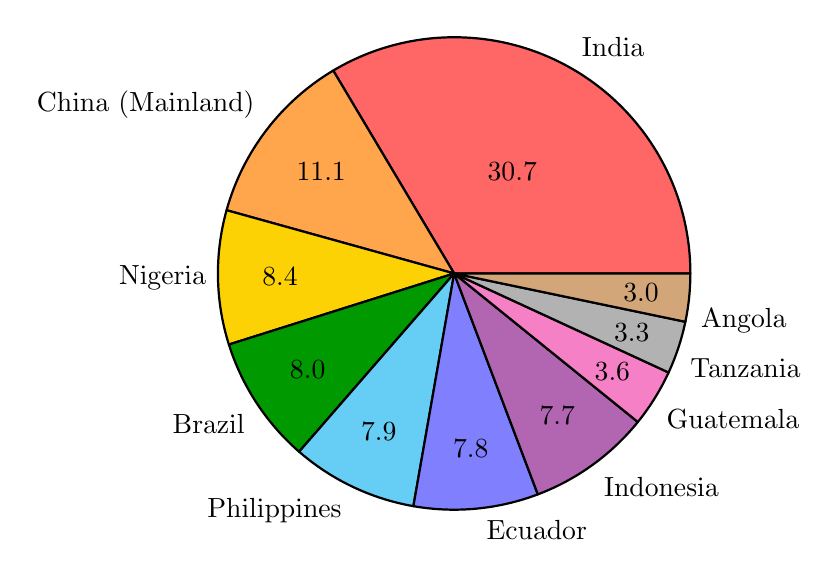
\begin{tikzpicture}
			\pie[
			color={red!60, orange!70, yellow!70!orange, green!60!black, cyan!60, blue!50, violet!60, magenta!50, gray!60, brown!70},
			sum=auto,
			line width=0.5pt
			]{
				30.7/India,
				11.1/China (Mainland),
				8.4/Nigeria,
				8.0/Brazil,
				7.9/Philippines,
				7.8/Ecuador,
				7.7/Indonesia,
				3.6/Guatemala,
				3.3/Tanzania,
				3.0/Angola
			}
		\end{tikzpicture}
	}
	\caption{Top ten largest banana producers globally (in metric tons, data from 2000--2023) \cite{voora2023global}.}
	\label{fig:banana_global} 
\end{figure}

\begin{figure}[!ht]
	\centering
	\resizebox{\columnwidth}{!}{%
		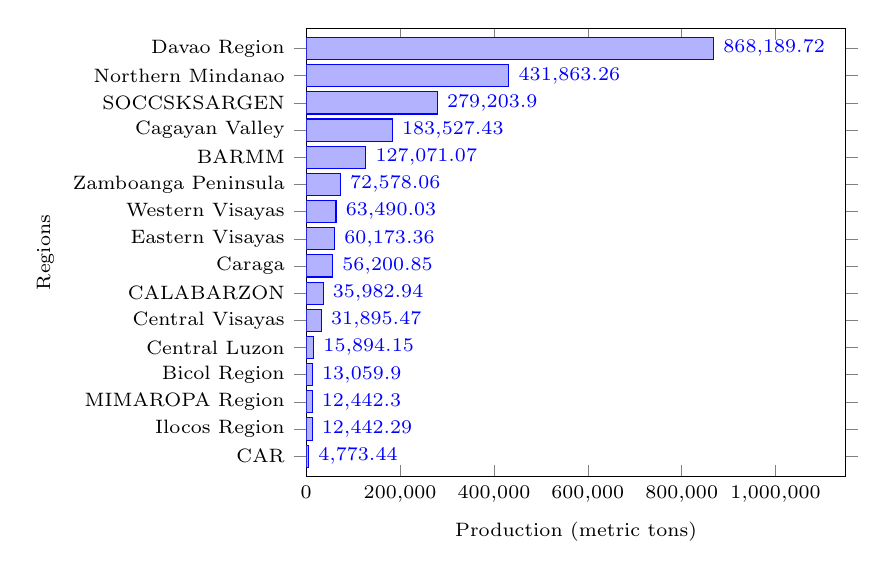
\begin{tikzpicture}
			\begin{axis}[
				xbar,
				bar width=8pt,
				symbolic y coords={
					CAR,
					Ilocos Region,
					MIMAROPA Region,
					Bicol Region,
					Central Luzon,
					Central Visayas,
					CALABARZON,
					Caraga,
					Eastern Visayas,
					Western Visayas,
					Zamboanga Peninsula,
					BARMM,
					Cagayan Valley,
					SOCCSKSARGEN,
					Northern Mindanao,
					Davao Region
				},
				ytick=data,
				yticklabel style={font=\scriptsize},
				xlabel={Production (metric tons)},
				ylabel={Regions},
				ylabel style={font=\scriptsize},
				xlabel style={font=\scriptsize},
				xmin=0,
				xmax=1150000,
				enlarge y limits=0.05,
				nodes near coords,
				every node near coord/.append style={font=\scriptsize, anchor=west, /pgf/number format/fixed},
				scaled x ticks=false,      
				tick label style={/pgf/number format/fixed, font=\scriptsize},
				]
				\addplot coordinates {
					(4773.44,CAR)
					(12442.29,Ilocos Region)
					(12442.30,MIMAROPA Region)
					(13059.90,Bicol Region)
					(15894.15,Central Luzon)
					(31895.47,Central Visayas)
					(35982.94,CALABARZON)
					(56200.85,Caraga)
					(60173.36,Eastern Visayas)
					(63490.03,Western Visayas)
					(72578.06,Zamboanga Peninsula)
					(127071.07,BARMM)
					(183527.43,Cagayan Valley)
					(279203.90,SOCCSKSARGEN)
					(431863.26,Northern Mindanao)
					(868189.72,Davao Region)
				};
			\end{axis}
		\end{tikzpicture}
	}
	\caption{Banana production by region in the Philippines (metric tons, 2023) \cite{PSABanana2023}.}
	\label{fig:banana-production}
\end{figure}

\begin{figure*}[htbp]
    \centering
    % First row
    \begin{minipage}[c]{0.48\linewidth}
        \centering
        \includegraphics[height=4cm, width=6cm]{Black-Sigatoka-infection.jpg}\\
        \parbox[t]{6cm}{\centering\small (a) Early dark streaks indicating infection.}
    \end{minipage}\hfill
    \begin{minipage}[c]{0.48\linewidth}
        \centering
        \includegraphics[height=4cm, width=6cm]{necroticlesions.jpg}\\
        \parbox[t]{6cm}{\centering\small (b) Black necrotic lesions and yellow halos.}
    \end{minipage}
    
    \vspace{1em}
    
    % Second row
    \begin{minipage}[c]{0.48\linewidth}
        \centering
        \includegraphics[height=4cm, width=6cm]{Black_Leaf_Streak1.jpg}\\
        \parbox[t]{6cm}{\centering\small (c) Macroscopic view of lesions, severe stage.}
    \end{minipage}\hfill
    \begin{minipage}[c]{0.48\linewidth}
        \centering
        \includegraphics[height=4cm, width=6cm]{1.jpg}\\
        \parbox[t]{6cm}{\centering\small (d) Leaves turn dark as tissues become waterlogged.}
    \end{minipage}
    
    \caption{Common symptoms of Black Sigatoka in banana leaves.}
    \label{fig:symptom_progression}
\end{figure*}

Given these pressing economic and farming challenges, researchers are now turning to computer-based methods, particularly computer vision and machine learning to help and improve traditional ways of detecting diseases.

\subsection{Automated Black Sigatoka Detection}
The study of Chaudhari and Patil \cite{chaudhari2020banana} aimed to develop an efficient automated system for the early identification of banana plant diseases (specifically Sigatoka, Cucumber Mosaic Virus (CMV), Bacterial Wilt, and Panama disease). The methodology involved capturing 618 digital images of banana leaves and preprocessing them by resizing to 400 × 600 pixels, enhancing with Adaptive Histogram Equalization, and converting to L*a*b* color space. Subsequently, K-means clustering was used to segment disease regions, from which color, shape, and texture features were extracted using a Gray Level Co-occurrence Matrix (GLCM). These features were then fed into a Support Vector Machine (SVM) classifier. The system achieved a classification accuracy of ~85\%, outperforming other classifiers.

Moreover, Escudero et al. \cite{escudero2021development} developed a mobile application using machine learning to detect Black Sigatoka disease in plantains. An image-processing algorithm enhanced disease patterns using a Gaussian filter and HSV color space transformation, which fed into an Ensemble Boosted Tree classifier achieving an efficiency of 80.58\%, and confusion matrices showed high accuracy (76.19\% for high severity), and user acceptance surveys revealed strongly positive feedback, with 87\% of users perceiving high effectiveness. 

Meanwhile, in a study by Evuri \cite{evuri2023banana} developed a machine learning system to identify banana leaf diseases (Sigatoka and Xanthomonas). The methodology followed the Knowledge Discovery Data Mining (KDD) process, utilizing a dataset of 1289 images of healthy leaves, Sigatoka, and Xanthomonas. After resizing the images to 224x224 pixels and sharpening using a 2D convolution filter, the system extracted features using GLCM and Neighbourhood Grey Tone Difference Matrix (NGTDM) techniques. These features were then classified using an SVM model, which achieved a high accuracy of 90\% in distinguishing between the diseases. 

\subsection{Automated Disease Detection of Other Crops}
In their study on leaf image-based plant disease identification, Ahmed et al. \cite{ahmad2021leaf} aimed to develop an efficient system suitable for mobile deployment to assist farmers in remote areas. Their methodology involved a two-stage process: first classifying leaves as healthy or diseased using a bag-of-features approach with Speeded Up Robust Features (SURF) features, then for diseased leaves, performing extensive preprocessing including background removal in HSV color space, bilateral filtering, and segmentation using Watershed algorithm and Otsu's method, followed by extraction of 28 hand-crafted color and texture features from GLCM, with feature standardization and selection via Forward Feature Selection before final classification using a Multi-Class SVM with cubic kernel. The system achieved exceptional results, with 99.48\% accuracy in healthy/diseased classification and 98.79\% accuracy in specific disease identification on 10-fold cross-validation, maintaining 91.40\% accuracy on an independent dataset.

Furthermore, in their study on diagnosing grape leaf diseases, Javidan et al. \cite{javidan2023diagnosis} aimed to develop a highly accurate and computationally efficient machine vision system for classifying black measles, black rot, leaf blight, and healthy leaves. Their methodology began with background removal using Canny edge detection and gray-level thresholding, followed by segmentation of the disease area using K-means clustering. A comprehensive set of features was then extracted from three color models (RGB, HSV, L*a*b*), with GLCM features proving most effective, and underwent feature dimension reduction via Principal Component Analysis (PCA) and selection using the Relief algorithm. A Multi-Class SVM with a linear kernel was used for classification, achieving a top accuracy of 98.97\% after PCA, while also demonstrating a significantly shorter processing time compared to deep learning models.

Meanshile, in the study of Jamjoom et al. \cite{Jamjoom2023}, they aims to develop an automated image processing system for four specific plant leaf diseases (\emph{Phytophthora infestans}, \emph{Fusarium graminearum}, \emph{Puccinia graminis}, and tomato yellow leaf curl). The methodology involves a multi-stage process beginning with image acquisition from the Plant Village dataset, followed by pre-processing where RGB images are converted to HSV format and enhanced using a median filter for noise reduction and smoothness, alongside Discrete Cosine Transform (DCT) for grayscale conversion. Image segmentation is then performed using an improved K-means clustering algorithm to isolate diseased regions, after which texture and color features are extracted utilizing Local Binary Pattern (LBP) and GLCM techniques. Finally, classification is executed with a Support Vector Machine (SVM) employing a radial basis function kernel. The key findings demonstrate that the proposed SVM-based model, supported by GLCM and LBP features, achieved a high average accuracy of 97.2\%, outperforming K-Nearest Neighbor (KNN) and Ensemble classifiers, which attained 80.2\% and 83.6\% accuracy, respectively.

Moreover, in their study on potato leaf disease detection, Iqbal and Talukder \cite{iqbal2020detection} aimed to develop an automatic system to identify and classify Early Blight, Late Blight, and healthy leaves to aid in crop protection. Their methodology involved preprocessing a dataset of 450 images from the PlantVillage database by resizing them and converting the color space from BGR to RGB and then to HSV. Image segmentation was performed by thresholding the HSV image to generate masks isolating the green (healthy) and brown (diseased) regions, from which global features for shape (Hu Moments), texture (Haralick Texture from GLCM), and color (Color Histogram) were extracted. These features were used to train seven different machine learning classifiers, with the Random Forest algorithm achieving the highest accuracy of 97\% on an 80-20 train-test split, outperforming others due to its ensemble decision-tree structure.

\subsection{Enhancement and Denoising Filters}
Across the studies, filters are employed as a critical pre-processing step to enhance image quality by reducing noise, which is essential for improving the accuracy of subsequent segmentation and classification tasks. In the Jamjoom et al. study \cite{Jamjoom2023}, a median filter is used during the pre-processing stage to remove noise and improve image smoothness after RGB images are converted to HSV format, thereby preparing the image for more effective segmentation via K-means clustering. 

The Mohanty and Tripathy \cite{mohanty2021filter} paper provides a comprehensive analysis of filtering techniques, systematically evaluating Mean, Gaussian, Wiener, and Median filters against different noise models (Gaussian, Salt and Pepper, Speckle, and Poisson) and quantitatively determining that the Wiener filter is best for Gaussian and Poisson noise, while the Median filter is most effective for Salt and Pepper noise, using MSE and PSNR as performance metrics. 

Similarly, the Jayashree and Sumalatha study \cite{jayashree2024filter} utilizes a combination of Gaussian and Wiener filters for pre-processing to normalize plant leaf images by minimizing noise and the Mean Square Error (MSE), which helps in creating a cleaner input for the Canny Region Extraction and subsequent deep learning model. 

Moreover, Yang et al. \cite{yang2025lightweight} employed an advanced denoising method based on the 2D Discrete Wavelet Transform (DWT) integrated with an adaptive thresholding strategy using the VisuShrink technique. This approach involved performing a four-level wavelet decomposition with the Haar wavelet to separate the image into low-frequency components, which capture the overall structure, and high-frequency components, which contain details and noise. The noise standard deviation was estimated from the highest frequency subband coefficients, and an adaptive threshold was dynamically calculated and applied using a soft thresholding function to suppress noise while preserving essential image details. After thresholding, the denoised image was reconstructed via the inverse 2D DWT, effectively reducing noise and enhancing feature clarity for subsequent deep learning analysis within their WaveLiteNet model.

\subsection{Synthesis of Identified Research Gaps}
Based on the comprehensive analysis of the studies, several significant research gaps emerge that highlight the current limitations and future directions in the field of plant disease detection using machine learning and image processing. Some of the identified gaps of the reviewed studies were addressed in this study.

A predominant gap across most studies is the limited generalizability and scalability of the developed models. Evuri \cite{evuri2023banana}, Chaudhari \& Patil \cite{chaudhari2020banana}, and Escudero et al. \cite{escudero2021development} all focused exclusively on banana diseases without testing their methodologies on other crops, raising questions about cross-crop applicability. Similarly, Iqbal \& Talukder \cite{iqbal2020detection} concentrated solely on potato diseases, while Ahmed et al. \cite{ahmad2021leaf}, despite working with multiple crops, showed a significant performance drop (from 98.79\% to 82.47\%) when tested on externally collected data, indicating poor generalization to real-world conditions. Furthermore, most studies lacked real-field validation, with laboratory-controlled conditions dominating the testing environments. The absence of mobile or real-time implementation in studies like Iqbal \& Talukder \cite{iqbal2020detection} and the computational heaviness noted in Ahmed et al. \cite{ahmad2021leaf} present practical deployment challenges. Dataset limitations were also prevalent, including class imbalances addressed only by Evuri \cite{evuri2023banana} using SMOTE, small dataset sizes particularly in Iqbal \& Talukder \cite{iqbal2020detection}, and insufficient diversity in disease stages and environmental conditions.

Another critical area of concern is the methodological and validation shortcomings. Most studies employed limited evaluation metrics, primarily focusing on accuracy without comprehensive analysis of precision, recall, or F1-scores across different disease classes, especially the study of Chaudhari \& Patil \cite{chaudhari2020banana} and Jamjoom et al. \cite{Jamjoom2023}. The segmentation approaches varied widely, with Chaudhari \& Patil \cite{chaudhari2020banana} using K-means clustering and Ahmed et al. \cite{ahmad2021leaf} employing Otsu's method and watershed algorithms, but none provided comparative analysis of segmentation effectiveness. Additionally, there was a consistent lack of severity quantification in disease detection, with only Escudero et al. \cite{escudero2021development} addressing multiple severity levels using the Fouré scale. The feature extraction methods, while diverse—ranging from GLCM and NGTDM in Evuri \cite{evuri2023banana} to DWT and FFT in Escudero et al. \cite{escudero2021development}, lacked standardized evaluation of their relative contributions to model performance. These methodological gaps are compounded by insufficient attention to computational efficiency and the absence of robustness testing against varying lighting conditions, image qualities, and background complexities that characterize real agricultural environments.

Table \ref{tab:disease-detection-comparison} summarizes the key methodologies and findings from the reviewed studies on plant disease detection.
\begin{table*}[htbp]
\centering
\begin{threeparttable}
\caption{\textbf{Summary of Plant Disease Detection Methods in Reviewed Studies}}
\label{tab:disease-detection-comparison}
\renewcommand{\arraystretch}{1.5}
\setlength{\tabcolsep}{4pt}
\begin{tabularx}{\textwidth}{
    >{\raggedright\arraybackslash}p{2.0cm}  % Study
    >{\centering\arraybackslash}p{2.6cm}  % Focus
    >{\centering\arraybackslash}p{3.0cm}  % Preprocessing
    >{\centering\arraybackslash}p{2.2cm}  % Features
    >{\centering\arraybackslash}p{3.8cm}  % Model
    >{\centering\arraybackslash}X         % Gaps
}
\toprule
\textbf{Author and Year} & \textbf{Crop \& Diseases} & \textbf{Preprocessing} & \textbf{Features} & \textbf{Model \& Accuracy} & \textbf{Limitations} \\
\midrule

Evuri (2022) \cite{evuri2023banana} & 
Banana: Sigatoka, Xanthomonas, Healthy & 
Resizing, Sharpening, SMOTE balancing & 
GLCM, NGTDM features & 
SVM + GLCM: 77.92\%;
SVM + NGTDM: 70.0\%;
SVM + GLCM + NGTDM: 90.38\% & 
Low accuracy, Single-crop focus, Limited conditions \\

Chaudhari \& Patil (2020) \cite{chaudhari2020banana} & 
Banana: Sigatoka, CMV, Bacterial Wilt & 
Resizing, Histogram Equalization, K-means & 
Color, GLCM texture & 
SVM (Linear): Overall 85\%, Black Sigatoka: 84\% & 
Lower accuracy, No cross-validation, Limited diseases \\

Escudero et al. (2020) \cite{escudero2021development} & 
Banana: Black Sigatoka (4 levels) & 
Gaussian filtering, HSV conversion, Contrast enhancement & 
DWT, FFT, Histogram & 
Ensemble Trees: 80.58\%\pm 1.05\% & 
Moderate accuracy, Single disease, No multi-crop validation \\

Iqbal \& Talukder (2021) \cite{iqbal2020detection} & 
Potato: Early/Late Blight, Healthy & 
Resizing, HSV conversion, Thresholding & 
Hu Moments, Haralick, Color & 
Random Forest: 97\% & 
Single crop focus, Small dataset \\

Ahmed et al. (2021) \cite{ahmad2021leaf} & 
14 crops, 26 diseases + healthy & 
Background removal, Otsu, Watershed & 
Color Moments, 22 GLCM features & 
SVM (Cubic): 98.79\% (CV) 82.47\% (external) & 
Performance drop on external data, No severity levels \\

Javidan et al. (2023) \cite{javidan2023diagnosis} & 
Grape: 3 diseases + healthy & 
Background/shadow removal, K-means & 
GLCM, LBP, HOG, Multi-color & 
SVM (Linear): 98.97\% & 
Feature effectiveness analysis provided \\

Jamjoom et al. (2023) \cite{Jamjoom2023} & 
Multiple crops: 4 diseases & 
DCT conversion, Median filter, K-means & 
GLCM, LBP, HSV & 
SVM (RBF): 97.2\% & 
Limited to specific viral diseases \\

\bottomrule
\end{tabularx}
\begin{tablenotes}
\footnotesize
\item \textit{Abbreviations: GLCM: Gray Level Co-occurrence Matrix; NGTDM: Neighbouring Grey Tone Difference Matrix; SVM: Support Vector Machine; DWT: Discrete Wavelet Transform; FFT: Fast Fourier Transform; SMOTE: Synthetic Minority Over-sampling Technique; CMV: Cucumber Mosaic Virus; CV: Cross-Validation}
\end{tablenotes}
\end{threeparttable}
\end{table*}

%################################################

\begin{table*}[htbp]
\centering
\small
\begin{threeparttable}
\caption{\textbf{Summary of Denoising Filters in Reviewed Studies}}
\label{tab:denoising-comparison}
\renewcommand{\arraystretch}{1.5}
\setlength{\tabcolsep}{3pt}
\begin{tabularx}{\textwidth}{
    >{\raggedright\arraybackslash}p{2.0cm}
    >{\centering\arraybackslash}p{3.5cm}
    >{\centering\arraybackslash}p{2.5cm}
    >{\centering\arraybackslash}p{3.0cm}
    >{\centering\arraybackslash}p{3.0cm}
    >{\centering\arraybackslash}X
}
\toprule
\textbf{Author and Year} & \textbf{Objective} & \textbf{Filters} & \textbf{Method} & \textbf{Equations} & \textbf{Results} \\
\midrule

Jamjoom et al. (2023) \cite{Jamjoom2023} & 
Remove noise and improve image smoothness & 
Median Filter & 
K-Means, GLCM+LBP, SVM & 
Median: $g(x, y) = \text{median} \{ f(x - i, y - j) \mid (i, j) \in W \}$ &
97.2\% accuracy, Beat KNN (80.2\%) \\

Mohanty \& Tripathy (2021) \cite{mohanty2021filter} & 
Evaluate Mean, Gaussian, Wiener, and Median filters against different noise models & 
Mean, Gaussian, Wiener, Median & 
MSE/PSNR metrics, Noise analysis & 
Mean: $g(x, y) = \frac{1}{mn} \sum_{(i, j) \in W} f(x - i, y - j)$ & 
Wiener: Gaussian/Poisson, Median: Salt/Pepper \\

Jayashree \& Sumalatha (2024) \cite{jayashree2024filter} & 
Normalize plant leaf images by minimizing noise & 
Gaussian, Wiener filters & 
ResNet-50, CRE, MRTS & 
Wiener: $\hat{F}(u, v) = \left[ \frac{1}{H(u, v)} \cdot \frac{|H(u, v)|^2}{|H(u, v)|^2 + K} \right] \times G(u, v)$ & 
95.1\% Accuracy, 96.5\% Precision \\

Yang et al. (2025) \cite{yang2025lightweight} & 
Reduce noise and enhancing feature clarity & 
2D DWT with VisuShrink & 
WaveLiteNet, MobileNetV3, CBAM & 
Wavelet Approx.: $C_{LL}(i, j) = \sum_{m} \sum_{n} f(m, n) h(2i - m) h(2j - n)$ & 
98.70\% accuracy, 25\% fewer parameters \\

\bottomrule
\end{tabularx}
\begin{tablenotes}
\footnotesize
\item \textit{Abbreviations: GLCM: Gray Level Co-occurrence Matrix; LBP: Local Binary Pattern; SVM: Support Vector Machine; DWT: Discrete Wavelet Transform; CBAM: Convolutional Block Attention Module; MSE: Mean Square Error; PSNR: Peak Signal-to-Noise Ratio}
\end{tablenotes}
\end{threeparttable}
\end{table*}


%################################################

\section{Methodology}\label{methodology}
\subsection{System Development Pipeline}
This study followed a structured multi-phase development pipeline designed to transform raw banana-leaf images into a standardized, noise-free, balanced, feature-rich dataset suitable for machine-learning classification of Black Sigatoka.

As shown in Fig. \ref{fig:systempipeline}, the pipeline begins with data inspection and data deduplication to ensure that the dataset is clean, with redundant data removed. Next, the data is standardized and denoised to remove any unwanted noise, ensuring that the features are consistent and reliable for analysis. The extraction phase selects important features, and masking is used to focus on key parts of the data, particularly for image-based tasks. The Region of Interest (ROI) extraction further isolates relevant areas of interest. After this, the data is organized and balanced to ensure that all categories or classes are equally represented for fair training. Then, the dataset undergoes feature extraction, and the model parameters are optimized through hyperparameter tuning for better performance.

\begin{figure*}
    \centering
    \includegraphics[width=0.6\linewidth]{systempipeline2.png}
    \caption{System Development Pipeline}
    \label{fig:systempipeline}
\end{figure*}

\subsection{System Architecture}
The architecture diagram illustrated in Fig. \ref{fig:systemarchitecture} represents the structured flow of the system components. It begins with data acquisition, where data is collected from various sources (e.g., sensors, images). Once data is obtained, it moves through the data preprocessing stage, which includes tasks such as cleaning, filtering, and normalization. Afterward, the data is processed into meaningful insights through feature extraction and modeling, where the system analyzes and interprets data. Model training follows, using a variety of machine learning or deep learning techniques to create a predictive model. The model is then evaluated to assess its performance, making adjustments as necessary for optimization. This architecture allows for continuous learning and improvement by enabling an iterative process of training, evaluation, and refinement, ensuring that the system becomes increasingly effective over time.

\begin{figure*}
    \centering
    \includegraphics[width=0.8\linewidth]{systemarchitecture2.png}
    \caption{System Architecture}
    \label{fig:systemarchitecture}
\end{figure*}

\subsection{Data Acquisition}
The researchers collected a total number of 38,563 images from various sources that are publicly available. Composed of 22,749 raw and 15,814 augmented images, selection of images that were used in the study narrowed down to 18,277 images (consisting of 15,495 and 2,782 raw and augmented images, respectively). The composition of the multi-source dataset used in the study is summarised in Tables \ref{tab:datasetimagesummarypart1} and \ref{tab:datasetimagesummarypart2}.

\begin{table*}[htbp]
\centering
\begin{threeparttable}
\caption{\textbf{Composition of Multi-Source Dataset}}
\label{tab:datasetimagesummarypart1}
\renewcommand{\arraystretch}{1}

\begin{tabularx}{\textwidth}{
    >{\raggedright\arraybackslash}p{3cm}
    >{\centering\arraybackslash}p{1.2cm}
    >{\centering\arraybackslash}p{1.2cm}
    >{\centering\arraybackslash}p{1.2cm}
    >{\centering\arraybackslash}p{1.2cm}
    >{\centering\arraybackslash}p{1.4cm}
    >{\centering\arraybackslash}p{1.4cm}
    >{\centering\arraybackslash}p{1.4cm}
    >{\centering\arraybackslash}p{1.4cm}
    >{\centering\arraybackslash}X
}
\toprule
\textbf{Disease / Condition} &
\multicolumn{2}{c}{\textbf{Mduma, et al. (2022) \cite{mduma2022dataset}}} &
\multicolumn{2}{c}{\textbf{Medhi \& Deb (2022) \cite{medhi2022dataset}}} &
\multicolumn{2}{c}{\textbf{Arman (2023) \cite{arman2023dataset}}} &
\multicolumn{2}{c}{\textbf{Das, et al. (2025) \cite{das2025dataset}}} \\
\cmidrule(lr){2-3} \cmidrule(lr){4-5} \cmidrule(lr){6-7} \cmidrule(lr){8-9}
 & \textbf{Avail.} & \textbf{Used} & \textbf{Avail.} & \textbf{Used} & \textbf{Avail.} & \textbf{Used} & \textbf{Avail.} & \textbf{Used} & \\
\midrule

Black Sigatoka        & \centering 5,767 raw & \centering 5,767 raw & \centering 474 raw & \centering 0 & \centering 473 raw, 400 aug. & \centering 0 & \centering \ding{55} & \centering \ding{55} & \\
Healthy               & \centering 5,628 raw & \centering 5,152 raw & \centering \ding{55} & \centering \ding{55} & \centering 129 raw, 400 aug. & \centering 0 & \centering 1,057 raw, 1,057 aug. & \centering 0 & \\
Banana Skipper Damage & \centering \ding{55} & \centering \ding{55} & \centering \ding{55} & \centering \ding{55} & \centering \ding{55} & \centering \ding{55} & \centering 17 raw, 1,057 aug.  & \centering 17 raw & \\
Boron Deficiency      & \centering \ding{55} & \centering \ding{55} & \centering \ding{55} & \centering \ding{55} & \centering \ding{55} & \centering \ding{55} & \centering \ding{55} & \centering \ding{55} & \\
Calcium Deficiency    & \centering \ding{55} & \centering \ding{55} & \centering \ding{55} & \centering \ding{55} & \centering \ding{55} & \centering \ding{55} & \centering \ding{55} & \centering \ding{55} & \\
Chewing Insect Damage & \centering \ding{55} & \centering \ding{55} & \centering \ding{55} & \centering \ding{55} & \centering \ding{55} & \centering \ding{55} & \centering 53 raw, 1,057 aug. & \centering 53 raw & \\
Cordana               & \centering \ding{55} & \centering \ding{55} & \centering \ding{55} & \centering \ding{55} & \centering 900 raw, 400 aug. & \centering \ding{55} & \centering \ding{55} & \centering \ding{55} & \\
Fusarium Wilt         & \centering 4,697 raw & \centering 980 raw & \centering 102 raw & \centering 0 & \centering \ding{55} & \centering \ding{55} & \centering 54 raw, 1,057 aug. & \centering 0 & \\
Insect Pest           & \centering \ding{55} & \centering \ding{55} & \centering \ding{55} & \centering \ding{55} & \centering \ding{55} & \centering \ding{55} & \centering \ding{55} & \centering \ding{55} & \\
Iron Deficiency       & \centering \ding{55} & \centering \ding{55} & \centering \ding{55} & \centering \ding{55} & \centering \ding{55} & \centering \ding{55} & \centering \ding{55} & \centering \ding{55} & \\
Magnesium Deficiency  & \centering \ding{55} & \centering \ding{55} & \centering \ding{55} & \centering \ding{55} & \centering \ding{55} & \centering \ding{55} & \centering \ding{55} & \centering \ding{55} & \\
Manganese Deficiency  & \centering \ding{55} & \centering \ding{55} & \centering \ding{55} & \centering \ding{55} & \centering \ding{55} & \centering \ding{55} & \centering \ding{55} & \centering \ding{55} & \\
Moko                  & \centering \ding{55} & \centering \ding{55} & \centering \ding{55} & \centering \ding{55} & \centering \ding{55} & \centering \ding{55} & \centering \ding{55} & \centering \ding{55} & \\
Pestalotiopsis        & \centering \ding{55} & \centering \ding{55} & \centering \ding{55} & \centering \ding{55} & \centering 173 raw, 400 aug. & \centering 173 raw, 330 aug. & \centering \ding{55} & \centering \ding{55} & \\
Potassium Deficiency  & \centering \ding{55} & \centering \ding{55} & \centering 1,530 raw & \centering 372 raw & \centering \ding{55} & \centering \ding{55} & \centering \ding{55} & \centering \ding{55} & \\
Sulphur Deficiency    & \centering \ding{55} & \centering \ding{55} & \centering \ding{55} & \centering \ding{55} & \centering \ding{55} & \centering \ding{55} & \centering \ding{55} & \centering \ding{55} & \\
Zinc Deficiency       & \centering \ding{55} & \centering \ding{55} & \centering \ding{55} & \centering \ding{55} & \centering \ding{55} & \centering \ding{55} & \centering \ding{55} & \centering \ding{55} & \\

\midrule
\textbf{Total Images} & \centering 16,092 raw & \centering 11,899 raw & \centering 2,160 raw & \centering 372 raw & \centering 1,675 raw, 1,600 aug. & \centering 173 raw, 330 aug. & \centering 1,181 raw, 4,228 aug. & \centering 70 raw & \\
\bottomrule
\end{tabularx}

\begin{tablenotes}
\footnotesize
\textit{\ding{55} – Class not available in the dataset source.
Avail. – Available images in the source dataset.
Used – Actual count used in the study.
aug. – Augmentation of raw images.}
\end{tablenotes}

\end{threeparttable}
\end{table*}

\begin{table*}[htbp]
\centering
\begin{threeparttable}
\caption{\textbf{Composition of Multi-Source Dataset (Continuation)}}
\label{tab:datasetimagesummarypart2}
\renewcommand{\arraystretch}{0.5}

\begin{tabularx}{\textwidth}{
    >{\centering\arraybackslash}p{2.5cm}
    >{\centering\arraybackslash}p{2cm}
    >{\centering\arraybackslash}p{2.5cm}
    >{\centering\arraybackslash}p{2.5cm}
    >{\centering\arraybackslash}p{3cm}
    >{\centering\arraybackslash}p{3cm}
}
\toprule
\multicolumn{2}{c}{\textbf{Kapadnis (2023) \cite{kapadnis2023dataset}}} &
\multicolumn{2}{c}{\textbf{Sunitha, et al. (2023/2025) \cite{sunitha2025dataset}}} &
\multicolumn{2}{c}{\textbf{Total}} \\
\cmidrule(lr){1-2} \cmidrule(lr){3-4} \cmidrule(lr){5-6}
\textbf{Avail.} & \textbf{Used} & \textbf{Avail.} & \textbf{Used} & \textbf{Avail.} & \textbf{Used} & \\
\midrule

\centering 67 raw, 469 aug. & \centering 0 & \centering \ding{55} & \centering 0 & \centering 6,781 raw, 869 aug. & \centering 5,767 raw & \\
\centering 86 raw, 602 aug. & \centering 0 & \centering 950 raw, 950 aug. & \centering 0 & \centering 7,850 raw, 3,009 aug. & \centering 5,152 raw & \\
\centering \ding{55} & \centering \ding{55} & \centering \ding{55} & \centering \ding{55} & \centering 17 raw, 1,057 aug. & \centering 17 raw & \\
\centering \ding{55} & \centering \ding{55} & \centering 100 raw, 800 aug. & \centering 100 raw, 73 aug. & \centering 100 raw, 800 aug. & \centering 100 raw, 73 aug. & \\
\centering \ding{55} & \centering \ding{55} & \centering 440 raw, 880 aug. & \centering 440 raw, 350 aug. & \centering 440 raw, 880 aug & \centering 440 raw, 350 aug. & \\
\centering \ding{55} & \centering \ding{55} & \centering \ding{55} & \centering \ding{55} & \centering 53 raw, 1,057 aug. & \centering 53 raw & \\
\centering \ding{55} & \centering \ding{55} & \centering \ding{55} & \centering \ding{55} & \centering 900 raw, 400 aug. & \centering 900 raw & \\
\centering 41 raw, 287 aug. & \centering 0 & \centering \ding{55} & \centering \ding{55} & \centering 4,894 raw, 1,344 aug. & \centering 980 raw & \\
\centering 86 raw, 688 aug. & \centering \ding{55} & \centering \ding{55} & \centering \ding{55} & \centering 86 raw, 688 aug. & \centering 86 raw, 688 aug. & \\
\centering \ding{55} & \centering \ding{55} & \centering 86 raw, 860 aug. & \centering 86 raw, 65 aug. & \centering 86 raw, 860 aug. & \centering 86 raw, 65 aug. & \\
\centering \ding{55} & \centering \ding{55} & \centering 160 raw, 800 aug. & \centering 160 raw, 110 aug. & \centering 160 raw, 800 aug. & \centering 160 raw, 110 aug. & \\
\centering \ding{55} & \centering \ding{55} & \centering 24 raw, 840 aug. & \centering 24 raw & \centering 24 raw, 840 aug. & \centering 24 raw & \\
\centering 55 raw, 440 aug. & \centering 55 raw, 440 aug. & \centering \ding{55} & \centering \ding{55} & \centering 55 raw, 440 aug. & \centering 55 raw, 440 aug. & \\
\centering \ding{55} & \centering \ding{55} & \centering \ding{55} & \centering \ding{55} & \centering 173 raw, 400 aug. & \centering 173 raw, 330 aug. & \\
\centering \ding{55} & \centering \ding{55} & \centering 210 raw, 840 aug. & \centering 0 & \centering 1,740 raw, 840 aug. & \centering 372 raw & \\
\centering \ding{55} & \centering \ding{55} & \centering 730 raw, 730 aug. & \centering 730 raw, 428 aug. & \centering 730 raw, 730 aug. & \centering 730 raw, 428 aug. & \\
\centering \ding{55} & \centering \ding{55} & \centering 400 raw, 800 aug. & \centering 400 raw, 298 aug. & \centering 400 raw, 800 aug. & \centering 400 raw, 298 aug. & \\

\midrule
\centering 335 raw, 2,486 aug. & \centering 55 raw, 440 aug. & \centering 3,100 raw, 6,660 aug. & \centering 1,940 raw, 1,324 aug. & \centering \textbf{22,749 raw, 15,814 aug.} & \centering \textbf{15,495 raw, 2,782 aug.} & \\
\bottomrule
\end{tabularx}

\begin{tablenotes}
\footnotesize
\textit{\ding{55} – Class not available in the dataset source.
Avail. – Available images in the source dataset.
Used – Actual count used in the study.
Total Used – Total count used in the study.
aug. – Augmentation of raw images.}
\end{tablenotes}

\end{threeparttable}
\end{table*}

The final number of images used in the study is due to the fact that the researchers created a third class ("Others") to have the system a robust learning aside from dominant number of classes "Black Sigatoka" and "Healthy". 

The "Others" class is intentionally heterogeneous and is used to represent a broad range of non–Black Sigatoka conditions. This provides diverse negative examples, which helps the classifier learn a more robust decision boundary between Black Sigatoka and non-Black Sigatoka leaves. The remainder of this paper will use these names "Healthy" for the healthy class of leaves, "BS" for Black Sigatoka class, and Others to refer to the heterogeneous class created.

The Others class comprises banana leaves with nutrient deficiencies, insect damage, and other non-Healthy and non-BS diseases, as shown in Tables \ref{tab:datasetimagesummarypart1} and \ref{tab:datasetimagesummarypart2}. Nutrient deficiencies include calcium, magnesium, potassium, iron, and zinc, which are commonly observed in banana plants under suboptimal soil conditions. Additionally, diseases such as Fusarium wilt, Moko, and Pestalotiopsis, alongside insect damage (e.g., chewing insect damage and insect pest), are grouped under this class. These categories, which represent a diverse range of conditions affecting banana plants, are crucial for diagnosing and managing plant health. Table \ref{tab:distributionthreemajor} shows the three major classes of the compiled dataset used in the study.

\begin{table}[htbp]
\centering
\begin{threeparttable}
\caption{\textbf{Unbalanced Dataset Distribution of Three Major Classes}}
\label{tab:distributionthreemajor}
\renewcommand{\arraystretch}{1.2}
\setlength{\tabcolsep}{6pt}
\begin{tabularx}{\linewidth}{
    >{\raggedright\arraybackslash}p{4.5cm}
    >{\centering\arraybackslash}X
    >{\centering\arraybackslash}X
}
\toprule
\textbf{Category / Folder} & \textbf{Images} & \textbf{Percentage} \\
\midrule
Healthy & 5,152 & 28.1\% \\
Black Sigatoka & 5,767 & 31.6\% \\
Others (Combined 15 Classes) & 7,358 & 40.3\% \\
\midrule
\textbf{Total} & \textbf{18,277} & \textbf{100\%} \\
\bottomrule
\end{tabularx}
\begin{tablenotes}
\footnotesize
\item \textit{Note: Other Diseases comprise: Banana Skipper Damage, Boron Deficiency, Calcium Deficiency, Chewing Insect Damage, Cordana, Fusarium Wilt, Insect Pest, Iron Deficiency, Magnesium Deficiency, Manganese Deficiency, Moko Disease, Pestalotiopsis, Potassium Deficiency, Sulphur Deficiency, Yellow Sigatoka, and Zinc Deficiency.}
\end{tablenotes}
\end{threeparttable}
\end{table}

However, it is evident that Table \ref{tab:distributionthreemajor} is an unbalanced dataset. To address this, a balanced dataset was created for model training, considering BS count, 5,767, as the target count for all major classes. The balanced version employed random undersampling of the majority Others class and applied data augmentation techniques to Healthy class to ensure equal representation across all three major categories. This approach resulted in each class containing exactly 5,767 images, totaling around 17,301 images in the balanced training set (see Table \ref{tab:distributionthreemajorbalanced}). The balanced distribution mitigates potential model bias toward overrepresented classes and improves generalization performance across all disease categories.

\begin{table}[htbp]
\centering
\begin{threeparttable}
\caption{\textbf{Balanced Dataset Distribution of Three Major Classes}}
\label{tab:distributionthreemajorbalanced}
\renewcommand{\arraystretch}{1.2}
\setlength{\tabcolsep}{6pt}
\begin{tabularx}{\linewidth}{
    >{\raggedright\arraybackslash}p{4.5cm}
    >{\centering\arraybackslash}X
    >{\centering\arraybackslash}X
}
\toprule
\textbf{Category / Folder} & \textbf{Images} & \textbf{Percentage} \\
\midrule
Healthy & 5,767 & ~33.3\% \\
Black Sigatoka & 5,767 & ~33.3\% \\
Others (Combined 15 Classes) & 5,767 & ~33.3\% \\
\midrule
\textbf{Total} & \textbf{18,277} & \textbf{~100\%} \\
\bottomrule
\end{tabularx}
\begin{tablenotes}
\footnotesize
\item \textit{Note: Other Diseases comprise: Banana Skipper Damage, Boron Deficiency, Calcium Deficiency, Chewing Insect Damage, Cordana, Fusarium Wilt, Insect Pest, Iron Deficiency, Magnesium Deficiency, Manganese Deficiency, Moko Disease, Pestalotiopsis, Potassium Deficiency, Sulphur Deficiency, Yellow Sigatoka, and Zinc Deficiency.}
\end{tablenotes}
\end{threeparttable}
\end{table}

The main contributor of the compiled dataset is the Nelson Mandela African Institute of Science and Technology, which provided a dataset of images captured from the Harvard Dataverse \cite{mduma2022dataset}. This dataset contains high-quality images of banana leaves affected by various diseases, such as BS and Fusarium Wilt, contributing significantly to the study of banana plant health. Another major contributor is the Medhi and Deb dataset \cite{medhi2022dataset}, which includes images captured using a Mendeley platform. It focuses on diseases like Fusarium Wilt and BS, and potassium deficiencies. Additionally, Das et al. \cite{das2025dataset} contributed dataset which covers a broad spectrum of banana leaf diseases, including healthy leaves. The Images of Nutrient Deficient Banana Plant Leaves dataset by Sunitha et al. \cite{sunitha2025dataset} includes data on nutrient deficiencies like zinc, iron, and calcium, crucial for understanding plant nutrition and its impact on banana crops. These datasets, as summarized in the Table \ref{tab:datasetreferences}, provide key references for training models to detect BS vs. Healthy vs. Non-BS diseases.

\begin{table*}[htbp]
\centering
\begin{threeparttable}
\caption{\textbf{Summary of Dataset References Used in the Study}}
\label{tab:datasetreferences}
\renewcommand{\arraystretch}{1.25}
\begin{tabularx}{\textwidth}{
    >{\raggedright\arraybackslash}p{1.7cm}  % Author
    >{\centering\arraybackslash}p{2.7cm}  % Dataset Name
    >{\centering\arraybackslash}p{1.3cm}  % Platform
    >{\centering\arraybackslash}p{1.3cm}  % Total Images
    >{\centering\arraybackslash}p{1.2cm}  % Image Size Pixel
    >{\centering\arraybackslash}p{1.0cm}  % Format
    >{\centering\arraybackslash}p{1.3cm}  % Size (Bytes)
    >{\centering\arraybackslash}X         % Key Classes
}
\toprule
\textbf{Author} &
\textbf{Dataset Name} &
\textbf{Platform} &
\textbf{Total Image Count} &
\textbf{Image Size} &
\textbf{Format} &
\textbf{Size (Bytes)} &
\textbf{Key Classes Covered} \\
\midrule

Mduma, et al. (2022) \cite{mduma2022dataset} &
The Nelson Mandela African Institution of Science and Technology Bananas Dataset &
Harvard Dataverse &
16,092 raw &
1024$\times$768 &
JPEG &
7.7 GB &
Black Sigatoka, Healthy, Fusarium Wilt \\

\addlinespace

Medhi \& Deb (2022) \cite{medhi2022dataset} &
PSFD-Musa Dataset &
Mendeley Data &
8000 raw &
256$\times$256 &
JPEG &
16.5 MB &
Potassium Deficiency, Bacterial Soft Rot, Banana Fruit Scarring Beetle, Black Sigatoka, Panama disease, etc. \\

\addlinespace

Arman (2023) \cite{arman2023dataset} &
Banana Leaf Spot Diseases Dataset &
Kaggle &
937 raw, 1600 aug. &
224$\times$224 &
JPEG &
40.05 MB &
Black Sigatoka, Cordana, Pestalotiopsis \\

\addlinespace

Das, et al. (2025) \cite{das2025dataset} &
Banana and Banana Leaf Dataset for Classification and Disease Detection &
Mendeley Data &
2375 raw, 9513 aug. &
1000\times750 &
JPEG &
329 MB &
Banana Skipper Damage, Black Sigatoka, Chewing Insect Damage, Healthy Banana, Healthy, Panama Wilt Disease, etc. \\

\addlinespace

Kapadnis (2023) \cite{kapadnis2023dataset} &
Banana Disease Recognition Dataset &
Kaggle &
408 raw, 2856 aug. &
512\times512 &
JPEG &
127.27 MB &
Healthy, Bract Mosaic Virus Disease, Black Sigatoka, Insect Pest Diseases, Moko Disease, Panama Disease \\

\addlinespace

Sunitha, et al. (2023/2025) \cite{sunitha2025dataset} &
Images of Nutrient Deficient Banana Plant Leaves &
Mendeley Data &
3950 raw, 7500 aug. &
255\times255 &
JPEG/PNG &
157 MB &
Healthy and Nutrient Deficiencies (Boron, Calcium, Iron, Potassium, Manganese, Magnesium, Sulphur and Zinc) \\

\bottomrule
\end{tabularx}


\begin{tablenotes}
\footnotesize
\textit{aug. – Augmentation of raw images.}
\end{tablenotes}

\end{threeparttable}

\end{table*}

\begin{figure*}[htbp]
    \centering
    % Row 1: Black Sigatoka, Healthy, and major diseases/insect damage
    \begin{minipage}[c]{0.18\textwidth}
        \centering
        \includegraphics[height=3cm, width=3cm]{Representation/bs.jpg}\\
        \parbox[t]{3cm}{\centering\small (a) Black Sigatoka}
    \end{minipage}\hfill
    \begin{minipage}[c]{0.18\textwidth}
        \centering
        \includegraphics[height=3cm, width=3cm]{Representation/healthy.jpg}\\
        \parbox[t]{3cm}{\centering\small (b) Healthy}
    \end{minipage}\hfill
    \begin{minipage}[c]{0.18\textwidth}
        \centering
        \includegraphics[height=3cm, width=3cm]{bananaskipper2.jpg}\\
        \parbox[t]{3cm}{\centering\small (c) Banana Skipper}
    \end{minipage}\hfill
    \begin{minipage}[c]{0.18\textwidth}
        \centering
        \includegraphics[height=3cm, width=3cm]{Representation/chewing.jpg}\\
        \parbox[t]{3cm}{\centering\small (d) Chewing Insect}
    \end{minipage}\hfill
    \begin{minipage}[c]{0.18\textwidth}
        \centering
        \includegraphics[height=3cm, width=3cm]{Representation/cordana.jpeg}\\
        \parbox[t]{3cm}{\centering\small (e) Cordana}
    \end{minipage}
    
    \vspace{1em}
    
    % Row 2: More diseases and insect damage
    \begin{minipage}[c]{0.18\textwidth}
        \centering
        \includegraphics[height=3cm, width=3cm]{Representation/fusarium.jpg}\\
        \parbox[t]{3cm}{\centering\small (f) Fusarium Wilt}
    \end{minipage}\hfill
    \begin{minipage}[c]{0.18\textwidth}
        \centering
        \includegraphics[height=3cm, width=3cm]{Representation/moko.jpg}\\
        \parbox[t]{3cm}{\centering\small (g) Moko Disease}
    \end{minipage}\hfill
    \begin{minipage}[c]{0.18\textwidth}
        \centering
        \includegraphics[height=3cm, width=3cm]{Representation/pestalotiopsis.jpeg}\\
        \parbox[t]{3cm}{\centering\small (h) Pestalotiopsis}
    \end{minipage}\hfill
    \begin{minipage}[c]{0.18\textwidth}
        \centering
        \includegraphics[height=3cm, width=3cm]{Representation/insectpest.jpg}\\
        \parbox[t]{3cm}{\centering\small (i) Insect Pest}
    \end{minipage}\hfill
    \begin{minipage}[c]{0.18\textwidth}
        \centering
        \includegraphics[height=3cm, width=3cm]{Representation/potassium.jpg}\\
        \parbox[t]{3cm}{\centering\small (j) Potassium}
    \end{minipage}
    
    \vspace{1em}
    
    % Row 3: Nutrient deficiencies
    \begin{minipage}[c]{0.18\textwidth}
        \centering
        \includegraphics[height=3cm, width=3cm]{Representation/magnesium.jpg}\\
        \parbox[t]{3cm}{\centering\small (k) Magnesium}
    \end{minipage}\hfill
    \begin{minipage}[c]{0.18\textwidth}
        \centering
        \includegraphics[height=3cm, width=3cm]{Representation/calcium.jpg}\\
        \parbox[t]{3cm}{\centering\small (l) Calcium}
    \end{minipage}\hfill
    \begin{minipage}[c]{0.18\textwidth}
        \centering
        \includegraphics[height=3cm, width=3cm]{Representation/sulphur.jpg}\\
        \parbox[t]{3cm}{\centering\small (m) Sulphur}
    \end{minipage}\hfill
    \begin{minipage}[c]{0.18\textwidth}
        \centering
        \includegraphics[height=3cm, width=3cm]{Representation/iron.jpg}\\
        \parbox[t]{3cm}{\centering\small (n) Iron}
    \end{minipage}\hfill
    \begin{minipage}[c]{0.18\textwidth}
        \centering
        \includegraphics[height=3cm, width=3cm]{Representation/zinc.jpg}\\
        \parbox[t]{3cm}{\centering\small (o) Zinc}
    \end{minipage}
    
    \vspace{1em}

     % Row 4: Remaining nutrient deficiencies
    \begin{minipage}[c]{0.18\textwidth}
        \centering
        \includegraphics[height=3cm, width=3cm]{Representation/boron.jpg}\\
        \parbox[t]{3cm}{\centering\small (p) Boron}
    \end{minipage}\hfill
    \begin{minipage}[c]{0.18\textwidth}
        \centering
        \includegraphics[height=3cm, width=3cm]{Representation/manganese.jpg}\\
        \parbox[t]{3cm}{\centering\small (q) Manganese}
    \end{minipage}\hfill
    \begin{minipage}[c]{0.18\textwidth}
        \centering
        \includegraphics[height=3cm, width=3cm]{Representation/white.png}\\
    \end{minipage}\hfill
    \begin{minipage}[c]{0.18\textwidth}
        \centering
        \includegraphics[height=3cm, width=3cm]{Representation/white.png}\\

    \end{minipage}\hfill
    \begin{minipage}[c]{0.18\textwidth}
        \centering
       \includegraphics[height=3cm, width=3cm]{Representation/white.png}\\
    \end{minipage}
    
    \caption{Visual representation of the 17 banana leaf condition classes used in the dataset, organized by category: (a-b) major classes, (c-i) diseases and insect damage, and (j-q) nutrient deficiencies.}
    \label{fig:all_classes}
\end{figure*}

%add also dataset pictures sa others classes

%add pictures sa balanced dataset split katong 3 figures

\begin{figure*}[htbp]
\centering
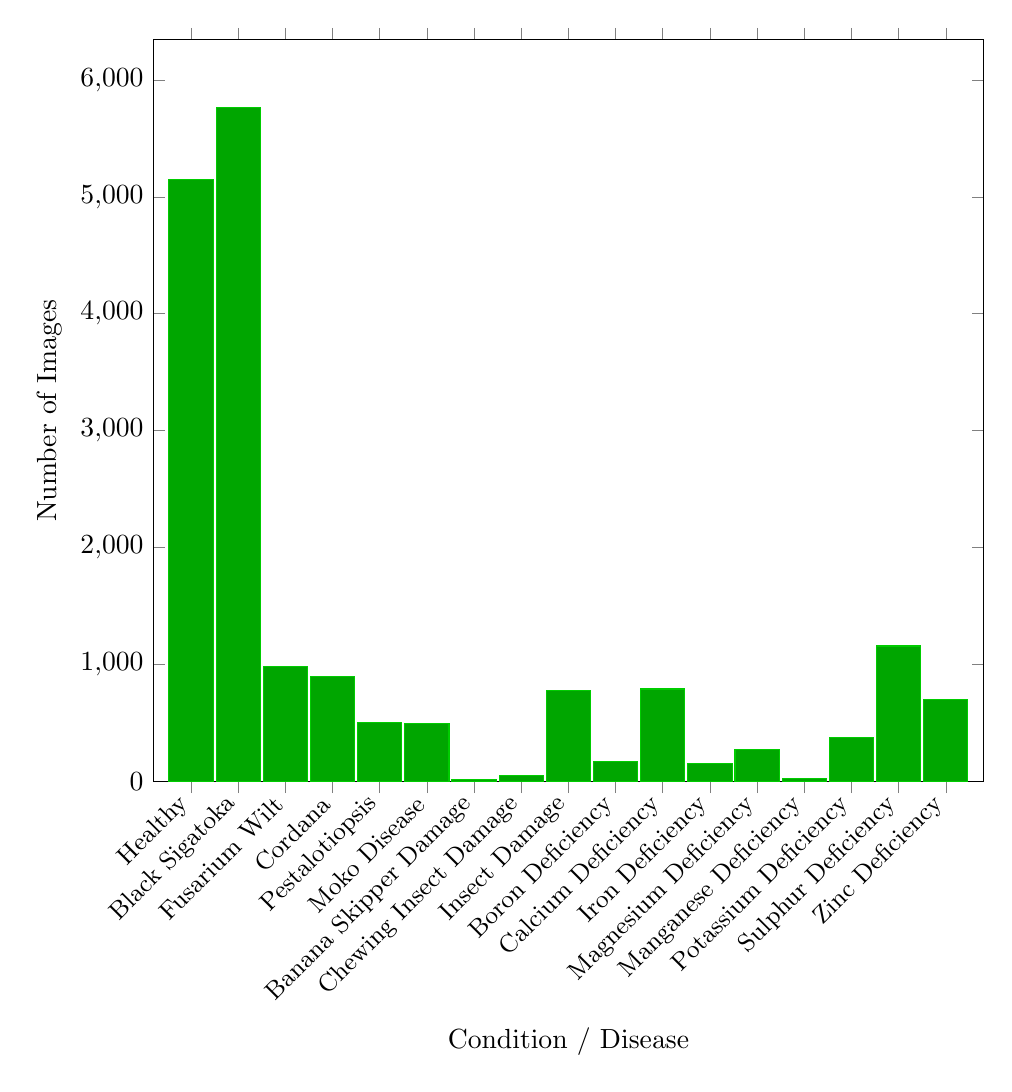
\begin{tikzpicture}
\begin{axis}[
    ybar,
    width=\textwidth,
    height=11cm, 
    enlarge x limits=0.05, 
    ylabel={Number of Images},
    xlabel={Condition / Disease},
    symbolic x coords={
        Healthy,Black Sigatoka,Fusarium Wilt,Cordana,
        Pestalotiopsis,Moko Disease,Banana Skipper Damage,
        Chewing Insect Damage,Insect Damage,Boron Deficiency,
        Calcium Deficiency,Iron Deficiency,Magnesium Deficiency,
        Manganese Deficiency,Potassium Deficiency,Sulphur Deficiency,
        Zinc Deficiency
    },
    xtick=data,
    xticklabel style={rotate=45, anchor=east, font=\small},
    bar width=16pt,    
    ymin=0,
]

\addplot[
    fill=green!65!black,
    draw=green!80!black
] coordinates {
    (Healthy,5152)
    (Black Sigatoka,5767)
    (Fusarium Wilt,980)
    (Cordana,900)
    (Pestalotiopsis,503)
    (Moko Disease,495)
    (Banana Skipper Damage,17)
    (Chewing Insect Damage,53)
    (Insect Damage,774)
    (Boron Deficiency,173)
    (Calcium Deficiency,790)
    (Iron Deficiency,151)
    (Magnesium Deficiency,270)
    (Manganese Deficiency,24)
    (Potassium Deficiency,372)
    (Sulphur Deficiency,1158)
    (Zinc Deficiency,698)
};
\end{axis}
\end{tikzpicture}
\caption{Expanded Dataset Distribution}
\end{figure*}

\begin{figure*}[htbp]
\centering
\begin{tikzpicture}
\begin{axis}[
    width=0.6\textwidth,
    height=8cm,
    ybar,
    bar width=15pt,
    enlargelimits=0.15,
    legend style={
        at={(0.5,-0.2)},
        anchor=north,
        legend columns=2,
        cells={anchor=west},
        draw=none
    },
    ylabel={Number of Images},
    symbolic x coords={Healthy, Black Sigatoka, Others},
    xtick=data,
    nodes near coords,
    nodes near coords align={above},
    every node near coord/.style={font=\small, color=black},
    ymajorgrids=true,
    grid style=dashed,
]

% Unbalanced dataset bars
\addplot[fill=red!60, pattern=north west lines, pattern color=red!80] coordinates {
    (Healthy, 5152)
    (Black Sigatoka, 5767)
    (Others, 7358)
};
% Balanced dataset bars
\addplot[fill=blue!60, pattern=crosshatch dots, pattern color=blue!80] coordinates {
    (Healthy, 5767)
    (Black Sigatoka, 5767)
    (Others, 5767)
};

\legend{Unbalanced Dataset, Balanced Dataset}

\end{axis}
\end{tikzpicture}
\caption{Comparison of class distribution between unbalanced and balanced datasets.}
\label{fig:dataset_balance_comparison}
\end{figure*}

% ============================================
% TABLE — Dataset Class Coverage Table (Thesis Version, Checkmarks Only)
% ===========================================

\begin{table*}[htbp]
\centering
\caption{Dataset Class Coverage}
\label{tab:dataset-coverage}
\renewcommand{\arraystretch}{1.25}
\begin{tabularx}{\textwidth}{
    >{\raggedright\arraybackslash}p{4cm}
    >{\centering\arraybackslash}p{1.8cm}
    >{\centering\arraybackslash}p{1.8cm}
    >{\centering\arraybackslash}p{1.8cm}
    >{\centering\arraybackslash}p{1.8cm}
    >{\centering\arraybackslash}p{1.8cm}
    >{\centering\arraybackslash}X}
\toprule
\textbf{Disease / Condition} &
\textbf{Medhi \& Deb (2022) \cite{medhi2022dataset}} &
\textbf{Arman (2023) \cite{arman2023dataset}} &
\textbf{Das, et al. (2025) \cite{das2025dataset}} &
\textbf{Kapadnis (2023) \cite{kapadnis2023dataset}} &
\textbf{Mduma, et al. (2022) \cite{mduma2022dataset}} &
\textbf{Sunitha, et al.(2023/2025) \cite{sunitha2025dataset}} \\
\midrule
Healthy                        & \checkmark & \checkmark & \checkmark & \checkmark & \checkmark &  \\ 
Black Sigatoka                 & \checkmark & \checkmark & \checkmark & \checkmark & \checkmark &  \\ 
Yellow Sigatoka                & \checkmark & \checkmark & \checkmark & \checkmark &             &  \\ 
Cordana              &            & \checkmark & \checkmark &             &             &  \\ 
Pestalotiopsis                 &            & \checkmark & \checkmark &             &             &  \\ 
Moko Disease                   &            & \checkmark & \checkmark &             &             &  \\ 
Fusarium Wilt (Panama)         &            &             &             &             & \checkmark &  \\ 
Xanthomonas Wilt (BXW)         &            &             &             &             & \checkmark &  \\ 
Banana Skipper Damage          &            &             &             & \checkmark &             &  \\ 
Chewing Insect Damage          &            &             &             &             &             &  \\ 
Banana Deficiency (General)    &            &             &             &             &             & \checkmark \\ 
Nutrient Deficiencies (Specific) &          &             &             &             &             & \checkmark \\ 
\bottomrule
\end{tabularx}

\vspace{4pt}
\small
\textit{Note. A checkmark (\checkmark) indicates that the corresponding dataset includes images for the specified disease or condition.}
\end{table*}


\subsection{Data Inspection and Analysis}\\
The initial phase focused on thoroughly examining the raw dataset to understand its overall structure, quality, and distribution. All image folders were scanned to determine how many files existed under each category and whether the dataset adhered to expected directory and naming conventions. This allowed identification of missing, mislabeled, or irregular data early in the pipeline. Class distributions were analyzed to detect imbalance, while visual inspection of sample images enabled identification of potential issues such as improper lighting, blur, shadows, and leaf deformation. Dataset size analysis helped determine the volume of data available for each class and guided subsequent steps such as augmentation and balancing.


\subsubsection{Dataset Structure Analysis}\\
The dataset structure analysis involved programmatically scanning all directories to confirm that images were correctly grouped into their respective class folders. This step verified the presence of three main categories—Healthy, Black Sigatoka, and Others—and ensured that each directory contained only image files. Structural analysis prevented downstream errors by identifying misplaced files, inconsistent naming patterns, or empty folders that could disrupt preprocessing. The process also included validating image extensions and counting files per class to ensure accurate dataset representation. This ensures that the dataset’s organizational integrity supports reproducible preprocessing and classification workflows.


\subsubsection{Dataset Distribution Visualization}\\
Dataset distribution visualization involved generating class-count plots to assess how many images belonged to each category. Visualizing the distribution allowed immediate identification of class imbalance, which is critical because imbalanced datasets can significantly bias machine-learning models. Class frequencies were analyzed mathematically using simple count functions, expressed as 
$n_c = |D_c|$ where $n_c$ is the number of images in class $c$. These counts were plotted as bar graphs to highlight disproportionate class representation. The visualization guided later augmentation strategies to ensure statistical fairness during training.

\subsubsection{Manual Sample Inspection}\\
Manual sample inspection involved visually reviewing randomly selected images from each class to assess their quality and suitability for training. This inspection step allowed identification of issues such as blur, excessive noise, occlusion, and poor lighting that automated validation might overlook. It also helped confirm whether images were correctly labeled, as mislabeling can significantly degrade model performance. Manual inspection also validated leaf visibility, color distribution, and disease appearance across samples, ensuring consistency for feature extraction. This step served as a qualitative verification before applying automated preprocessing and cleaning.


\subsubsection{Dataset Size Analysis}\\
Dataset size analysis quantified the total number of valid images and the number of samples per class to evaluate dataset adequacy for machine learning. A dataset size summary was computed using the formula

\begin{equation}
N_{\text{total}} \;=\; \sum_{c=1}^{C} n_c,
\end{equation}

where $N_\text{total}$ is the total dataset size and represents the number of images in class $c$. This analysis helped determine whether the dataset required augmentation or balancing to achieve acceptable sample diversity. Understanding dataset size also guided memory allocation and batch processing design during training. The results informed the scale and intensity of augmentation steps applied later in the pipeline.


\subsection{Data Cleaning and Deduplication}\\
This phase ensured that only valid, readable, and unique images were retained for downstream processing. Cleaning the dataset prevented corrupted or incorrect samples from negatively influencing feature extraction and model training. Deduplication ensured statistical fairness by removing repeated images that could bias the classifier. Noise filtering techniques improved the quality of the images by minimizing distortions that interfere with texture- and frequency-based feature extraction. Overall, this phase established a clean and consistent dataset foundation for subsequent analysis.

\subsubsection{Remove Corrupt Images}\\
Removing corrupt images was essential to prevent errors during preprocessing and feature extraction. Corrupt images were identified using automated file validation, where each image was loaded to determine if its pixel data could be successfully decoded. If an image failed to load or returned incomplete data, it was removed from the dataset. This step ensured that only valid numerical pixel matrices were included, preventing downstream failures in operations such as resizing, filtering, and segmentation. Formally, an image $I$ was considered valid if its decoded matrix satisfied

\begin{equation}
N_{\text{total}} \;=\; \sum_{c=1}^{C} n_c,
\end{equation}

Images failing this condition were classified as corrupt and excluded.

\subsubsection{Remove Exact Duplicates}\\
Exact duplicates were removed to prevent redundancy and sampling bias during training. Duplicate detection was performed using hashing functions, where each image’s binary representation was converted into a hash value. If two images shared the same hash $h(I_1)=h(I_2)$, they were assumed to be identical. This ensured that the model did not “see” the same image multiple times, which would otherwise inflate performance and reduce generalization. Deduplication also optimized storage efficiency and reduced unnecessary computational load during processing.

\subsubsection{Remove Non-Image Files}\\
This step ensured that only valid image formats entered the pipeline by filtering files based on extension and successful decoding. In real-world datasets, directories may contain .txt, .json, .db, or temporary files that could disrupt automated processing. Non-image files were detected by verifying file extensions and validating whether the file content could be read as pixel data. Any file failing these conditions was excluded. This validation ensured a clean dataset composed solely of analyzable images.

\subsubsection{Advanced Noise Filtering (Median → Wiener → Wavelet)}\\
A three-stage noise reduction pipeline was applied to enhance image quality and preserve critical texture features. Median filtering removed salt-and-pepper noise by replacing each pixel with the median of its neighborhood, mathematically defined as
\begin{equation}
I'(x,y) \;=\; \operatorname{median}\{ I(i,j)\},
\end{equation}

for all $(i,j)$ in a local window.
Wiener filtering adapted to local variance and minimized mean squared error using

\begin{equation}
I'(x,y) \;=\; \mu \;+\; \frac{\sigma^2 - \nu^2}{\sigma^2} \, ( I(x,y) - \mu ),
\end{equation}

where $\mu$ and $\sigma^2$ are local mean and variance and $v^2$ is noise variance.
Wavelet filtering decomposed images into frequency bands and suppressed high-frequency noise through thresholding:

\begin{equation}
W' \;=\; \operatorname{soft}(W, \lambda)
\end{equation}

This combination preserved edges while stabilizing intensity values for feature extraction.

\subsection{Data Preprocessing and Standardization}
\subsubsection{Standardize Image Sizes}\\
Standardizing image sizes ensured that all samples were represented by pixel matrices of consistent dimensions. Non-uniform image shapes cause inconsistencies in matrix operations such as convolution, frequency transforms, and texture computation. Each image was resized to a fixed resolution $H \times W$, expressed as

\begin{equation}
I' \;=\; \text{resize}(I, H, W).
\end{equation}

This normalization ensured that every sample contributed equally during feature extraction. Standardized sizes also simplified batch processing and reduced computational variability.

\subsubsection{Convert to RGB Format}\\
Converting all images to RGB ensured consistent color representation across the dataset. Since images may originate from various devices and formats—such as grayscale or RGBA—conversion standardized each image to three channels. The RGB conversion ensured that color-based features such as histograms and disease-specific ratios were computed consistently. Formally, each pixel was represented as

\begin{equation}
    I(x,y)=[R(x,y), G(x,y), B(x,y)]
.\end{equation}

This uniform color structure prevented channel mismatches during feature extraction.

\subsubsection{Calculate Normalization Parameters}\\
Normalization parameters—the global dataset mean and standard deviation—were computed to standardize pixel intensity values. These parameters ensured that lighting differences across images did not bias feature extraction. The mean and standard deviation were calculated as:

\begin{equation}
\mu \;=\; \frac{1}{N} \sum_{i=1}^{N} I_i,
\end{equation}
\begin{equation}
\sigma \;=\; \sqrt{ \frac{1}{N} \sum_{i=1}^{N} (I_i - \mu)^2 }.
\end{equation}

Pixel normalization was applied using

\begin{equation}
I' \;=\; \frac{I - \mu}{\sigma}.
\end{equation}
This improved algorithmic stability in downstream computations.

\subsection{Dataset Organization and Splitting}\\
This phase reorganized the cleaned dataset and prepared training, validation, and testing partitions. A clear 3-class structure—Healthy, Black Sigatoka, and Others—was established to support supervised classification. Stratified splitting ensured that class proportions remained consistent across all partitions. This prevented training bias and ensured performance metrics accurately represented the model’s ability to generalize.

\subsubsection{Create 3-Class Structure (Healthy, Black Sigatoka, Others)}\\
The dataset was grouped into three clearly defined classes to facilitate the supervised learning process. These categories reflected the study’s primary classification objectives. Organizing images into these classes ensured that labels were correctly aligned with visual features. The structure also supported consistent sampling during training and evaluation. This grouping served as the foundation for stratified splitting and performance analysis.

\subsubsection{Create Stratified Train/Validation/Test Splits}\\
Stratified splitting preserved the class distribution across training (70\%), validation (15\%), and testing (15\%) sets. Stratification ensured proportional representation of each class, computed as

\begin{equation}
    p_c= \frac{n_c}{N_\text{total}}.
\end{equation}
Sampling then maintained

\begin{equation}
    n_c,_k=p_c \times N_k,
\end{equation}

where $k$ denotes train, validation, or test partitions. This preserved statistical consistency across all splits and improved reliability of performance metrics.

\subsection{Class Imbalance Handling}\\
This phase addressed the natural imbalance in the dataset, where certain classes contained significantly more samples than others. Imbalanced datasets can bias machine-learning models to favor majority classes, leading to unreliable predictions for minority categories such as early-stage infection cases. By identifying imbalance early and applying corrective techniques, the study ensured that all classes contributed equally to training. This phase improved classifier robustness and prevented skewed model behavior. The steps included analyzing class statistics, augmenting minority samples, and matching class counts.

\subsubsection{Analyze Class Imbalance}\\
Class imbalance was analyzed by computing the number of samples per class and comparing these counts to determine proportional differences. This was quantified using the imbalance ratio (IR), expressed as

\begin{equation}
    IR_c = \frac{max(n_1, n_2, n_3}{n_c},
\end{equation}

where $n_c$ is the number of images in class $c$. A higher imbalance ratio indicates an underrepresented class. Visualization of sample distribution confirmed whether one or more classes required augmentation. This quantitative assessment provided the foundation for implementing corrective balancing methods.

\subsubsection{Augment Minority Class}\\
Minority classes were augmented using controlled image transformations that preserved medically relevant features while increasing sample diversity. Augmentation operations such as rotations, flips, translations, and color modifications expanded the dataset without altering disease appearance. Formally, augmentation can be represented as a transformation function

\begin{equation}
    I' = T (I, 0),
\end{equation}

where $T$ applies a parameterized transformation $0$ to image $I$. These transformations simulate natural variations in leaf orientation and lighting. Augmentation ensured that minority classes contributed equally during classifier training, preventing bias in learned decision boundaries.

\subsubsection{Balance All Classes to Match Black Sigatoka Count}\\
The final step involved adjusting all class counts to match the number of Black Sigatoka samples, which served as the target class reference. By equalizing sample counts, the study achieved a balanced dataset where each class had equivalent representation. This balancing reduced the risk of model overfitting toward majority classes and improved classification fairness. Formally, each class was expanded or trimmed to meet

\begin{equation}
n_c^* \;=\; \max(n_1,\, n_2,\, n_3).
\end{equation}

Balanced class distributions ensure that traditional machine-learning classifiers operate under uniform statistical conditions.

\subsection{Dataset Splitting (Balanced)}\\
After balancing the dataset, new stratified splits were created to ensure that the train–validation–test sets remained equally represented. This step ensured that the benefits of balancing were preserved across all dataset partitions. Balanced splitting improved evaluation reliability and prevented misleading performance metrics caused by accidental distribution shifts. This stage also generated metadata files documenting the final dataset composition.

\subsubsection{Create Stratified Splits from Balanced Dataset}\\
Stratified sampling was applied again, this time using the balanced dataset to ensure equal representation of classes across all partitions. The proportion of samples for each split was preserved using the formula

\begin{equation}
    n_c,_k=\frac{N_k}{N_\text{balanced}}n_c^*,
\end{equation}

where $N_k$ is the number of samples allocated for split $k$ and $n_c^*$ is the balanced class size. Stratification prevented accidental dominance of any class within a partition. The resulting splits maintained structural consistency required for fair model comparison.

\subsubsection{Analyze Split Distribution}\\
After generating the stratified splits, the distribution of samples across each partition was verified to confirm statistical consistency. Verification computed the proportion of each class in each split and checked whether it matched the expected distribution within a small tolerance. The class proportion in split $k$ is given by

\begin{equation}
    p_c,_k=\frac{n_c,_k}{N_k}.
\end{equation}

Any deviations were corrected by adjusting sampling indices. This ensured that training, validation, and testing sets reflected the same balanced structure.

\subsubsection{Visualize Splits}\\
Class distributions across the balanced splits were visualized using bar charts and summary plots. Visual inspection provided an intuitive check to confirm that each class was uniformly represented. Visualization complemented numerical verification, ensuring that no sampling error or imbalance occurred during the splitting process. Clear visualization also supports methodological transparency and reproducibility. This step validated the effectiveness of the balancing and stratification procedures.


\subsubsection{Create Split Metadata}\\
Metadata files were generated to document the filenames, labels, and partitions of all images in the balanced dataset. These metadata logs ensured that experiments could be reproduced exactly, even across different machines or researchers. A metadata table $M$ was generated containing rows of the form

\begin{equation}
    M_i=(\text{filename}_i, \text{class}_i, \text{split}_i).
\end{equation}

This structured information also facilitated batch loading during feature extraction. Metadata creation ensured full traceability of dataset organization.

\subsection{Feature Extraction for Traditional ML}\\
This phase extracted quantitative descriptors from each image to capture texture, color, structural, and frequency characteristics relevant to Black Sigatoka detection. Feature extraction transforms raw pixel data into mathematically meaningful representations that can be interpreted by machine-learning algorithms. The extracted features included texture-based descriptors such as GLCM and LBP, frequency-domain representations such as DWT and FFT, color histograms, Hu moments, and disease-specific indicators. Each feature type contributed complementary information, improving the classifier’s ability to differentiate Healthy, Black Sigatoka, and Other leaf conditions. Together, these features formed a comprehensive representation of leaf appearance.
\subsubsection{GLCM Texture Features}\\
Gray-Level Co-occurrence Matrix (GLCM) features were extracted to capture spatial relationships between pixel intensities, which are essential for distinguishing disease patterns. GLCM analyzes how often pairs of pixel intensities $(i,j)$ (i,j) occur at specific spatial offsets. From the co-occurrence matrix $P(i,j)$, P(i,j), several texture measures were computed, including contrast, homogeneity, energy, and correlation. For example, contrast was defined as

\begin{equation}
\text{Contrast} \;=\; \sum_{i=1}^{N} (i - j)^{2} \, P(i,j).
\end{equation}

while homogeneity was given by

\begin{equation}
\text{Homogeneity} \;=\; \sum_{i,j} \frac{P(i,j)}{1 + |i - j|}.
\end{equation}

These features captured the roughness and uniformity of leaf textures, which are altered significantly by Black Sigatoka lesions.


\subsubsection{LBP Texture Features}\\
Local Binary Patterns (LBP) captured micro-texture variations by comparing each pixel with its surrounding neighbors. For a given pixel $p$, LBP computes a binary pattern by thresholding its neighbors:

\begin{equation}
LBP(p) \;=\; \sum_{k=0}^{P-1} s(I_k - I_p)^2,
\end{equation}

where

\begin{equation}
s(x) =
\begin{cases}
1, & x \ge 0,\\
0, & x < 0.
\end{cases}
\end{equation}

This binary code reflects local texture differences, making LBP highly effective for identifying spot-like lesions characteristic of Black Sigatoka. Histograms of LBP codes were computed to summarize texture distributions. These descriptors provided strong discrimination between healthy smooth textures and infected rough patterns.


\subsubsection{Discrete Wavelet Transform (DWT) Features}\\
Discrete Wavelet Transform (DWT) decomposed images into multiple frequency sub-bands that captured both coarse and fine details. The DWT generated approximation coefficients (LL) and detail coefficients (LH, HL, HH), reflecting horizontal, vertical, and diagonal frequency components. Mathematically, DWT is expressed as

\begin{equation}
    W_s,_t=\sum_{k=0}I(x) \psi_s,_t(x),
\end{equation}

where $\psi_s,_t$ is the wavelet basis scaled by $s$ and translated by $t$. Statistical features such as mean, energy, and standard deviation were calculated from each sub-band. DWT helped differentiate between smooth healthy leaf regions and frequency-rich diseased areas.
\subsubsection{Fast Fourier Transform (FFT) Features}\\
Fast Fourier Transform (FFT) converted the image from spatial to frequency domain to highlight repetitive patterns caused by disease progression. FFT computes the frequency spectrum as

\begin{equation}
F(u,v) \;=\; \sum_{x,y} I(x,y)\, e^{-j 2\pi (u x + v y)/N}.
\end{equation}

Magnitude and phase components were analyzed, with emphasis on frequency magnitude:

\begin{equation}
|F(u,v)| \;=\; \sqrt{ \Re(F(u,v))^{2} \;+\; \Im(F(u,v))^{2} }.
\end{equation}

High-frequency energy often reflects rough or speckled structures associated with fungal lesions, while low-frequency content characterizes smooth leaf surfaces. FFT-derived statistics captured global frequency trends relevant to disease identification.

\subsubsection{Histogram Features}\\
Color histograms were computed across RGB and HSV channels to quantify color distribution in each image. Each histogram represented the frequency of pixel intensities within predefined bins:

\begin{equation}
    H_b=|{I(x,y)\in b}|,
\end{equation}

where $b$ denotes a histogram bin. These features captured variations in leaf coloration such as yellowing, browning, or dark streaks characteristic of infection. Normalized histograms were computed to ensure consistency across image sizes:

\begin{equation}
    H_b' = \frac{H_b}{\sum _b H_b} .
\end{equation}

Histograms provided stable color descriptors that complemented structural feature sets.

\subsubsection{Hu Moments}\\
Hu moments captured global shape characteristics derived from second-order image moments. Central moments were computed as

\begin{equation}
\mu_{pq} \;=\; \sum_{x} \sum_{y} (x - \bar{x})^{p} (y - \bar{y})^{q} I(x,y),
\end{equation}

followed by calculating seven invariant Hu moments $\phi_1,...,\phi_7.$ For example,

\begin{equation}
\phi_{1} \;=\; \eta_{20} \;+\; \eta_{02},
\end{equation}

\begin{equation}
\phi_{2} \;=\; (\eta_{20} \;-\; \eta_{02})^{2} \;+\; 4\,\eta_{11}^{2},
\end{equation}

where $\eta _{pq}$are normalized central moments. These descriptors are invariant to rotation, scaling, and translation, making them suitable for characterizing leaf shapes and deformation patterns associated with disease.

\subsubsection{Color Features}\\
Color features quantified pigmentation changes caused by Black Sigatoka, including shifts toward brown, black, or yellow. Pixel-level measures such as average RGB values were computed:

\begin{equation}
    \bar{C}=\frac{1}{N}\sum_{x,y}C(x,y),
\end{equation}

where $ C \in (R, G, B )$
. Additional ratios such as green-to-red (G/R) and brown intensity were extracted to characterize chlorosis and necrosis. These features captured global color trends that differ significantly among healthy leaves and infected ones. Color descriptors complemented texture-based features to improve classifier discrimination.

\subsubsection{Disease-Specific Features}\\
Disease-specific features targeted visual symptoms unique to Black Sigatoka, such as streak intensity, lesion darkness, and edge density. These metrics were computed using color segmentation masks, pixel intensity thresholds, and directional texture measures. For example, the dark lesion ratio was computed as

\begin{equation}
\text{DLR} \;=\; \frac{\left| I(x,y) < T_d \right|}{N},
\end{equation}

where $T_d$ is a disease threshold derived from dataset intensity histograms. By extracting quantitative indicators of disease severity, these features strengthened the classifier’s ability to recognize infection patterns.
\subsection{Feature Preprocessing and Selection}\\
This phase ensured that all extracted features were clean, consistent, and suitable for machine-learning classification. Raw feature vectors may contain redundant, constant, or missing values that negatively affect classifier performance, so preprocessing was necessary to standardize and optimize the feature set. Scaling, encoding, and feature selection techniques were used to ensure that the resulting feature vectors had meaningful variance, numerical stability, and discriminative power. These steps reduced dimensionality, removed noise, and improved training efficiency. The resulting feature matrix served as a high-quality input for the classifiers.

\subsubsection{Remove Constant Features}\\
Constant features were removed because they provide no discriminative power for classification and unnecessarily increase feature dimensionality. A feature $f$ is considered constant if

\begin{equation}
    \text{Var} f =0,
\end{equation}

meaning that all samples share identical values for that feature. Such features contribute nothing to model learning and can reduce computational efficiency. Removing them prevents algorithms from wasting processing time on uninformative data. This step ensured that the feature matrix consisted only of meaningful, variable descriptors.

\subsubsection{Handle Missing Values}\\
Missing feature values were identified and corrected to prevent errors during classifier training. Missing entries may arise from images where specific transformations fail, such as LBP computation on small patches or wavelet coefficients returning undefined values. Missing values were handled using imputation, typically by replacing them with the feature mean:

\begin{equation}
f_i' \;=\; \begin{cases}
f_i, & f_i \neq \emptyset,\\[6pt]
\mu_f, & f_i = \emptyset .
\end{cases}
\end{equation}

This ensured numerical completeness and prevented downstream algorithms from encountering invalid values. Proper handling of missing data maintained dataset integrity.

\subsubsection{Encode Labels}\\
Label encoding converted categorical class labels (Healthy, Black Sigatoka, Others) into numerical values for machine-learning compatibility. Each class label was mapped to an integer $y \in$ {0, 1, 2}, enabling computation of loss functions and classification metrics. Formally,

\begin{equation}
    y=E(label),
\end{equation}

where $E$ is the encoding function. Encoding ensured that all samples had machine-interpretable identifiers for supervised learning. This step allowed classifiers to process class information in a mathematically consistent manner.

\subsubsection{Scale Features}\\
Feature scaling standardized the numerical ranges of all features to ensure uniform contribution during training. Without scaling, features with larger numeric ranges can dominate distance-based metrics, especially for SVM and k-Nearest Neighbors. Standardization was performed using

\begin{equation}
    f_i'=\frac{f_i-\mu_f}{\sigma_f}
\end{equation}

where $\mu_f$ and $\sigma _f$ are the feature’s mean and standard deviation. Scaling stabilized gradient computations and improved model convergence. This ensured fair representation of all feature dimensions.

\subsubsection{Feature Selection (Random Forest, ANOVA, RFE)}\\
Multiple feature-selection techniques were used to retain only the most informative descriptors. Random Forest computed feature importance using impurity reduction, expressed as

\begin{equation}
    \Delta G=G_\text{parent}-(G_\text{left}+G_\text{right}),
\end{equation}

where $G$ denotes Gini impurity.
ANOVA evaluated features using F-scores:

\begin{equation}
    F=\frac{\text{Between-class variance}}{\text{Within-class variance}},
\end{equation}

Recursive Feature Elimination (RFE) iteratively removed the least important features based on classifier weights. Combining these techniques ensured stable, high-quality feature subsets and reduced dimensionality for optimal model performance.

\subsubsection{Create Testing Pipeline}\\
A unified feature-processing pipeline was constructed to ensure that new images undergo identical preprocessing steps as training samples. The pipeline combined feature extraction, scaling, feature selection, and classification into a single sequential process. Formally, the pipeline can be represented as

\begin{equation}
    P=C(S(F(I))),
\end{equation}

where $I$ is the input image, $F$ is feature extraction, $S$ is scaling and selection, and $C$ is classification. This ensured reproducibility and prevented preprocessing mismatches between training and deployment. The pipeline was saved for automated inference.
\subsection{Model Training with Traditional ML}\\
This phase involved training multiple classical machine-learning classifiers on the optimized feature set. Training procedures ensured that classifiers learned discriminative patterns derived from textures, colors, and frequency-domain representations. Cross-validation was used to evaluate generalization performance across multiple subsets of the training data. The best-performing model based on accuracy, consistency, and stability was selected for final evaluation. This ensured that the chosen classifier represented the most reliable model for deployment.

\subsubsection{Initialize Classifiers (SVM, Random Forest, Gradient Boosting, etc.)}\\
Several machine-learning classifiers were initialized to compare performance across different decision boundaries and learning mechanisms. Support Vector Machines (SVM) attempted to find the optimal separating hyperplane

\begin{equation}
    w^Tx+b=0,
\end{equation}

by maximizing margin distance.
Random Forest used an ensemble of decision trees, improving stability through bagging.
Gradient Boosting sequentially minimized the loss function by adding trees that corrected previous errors.
Initializing diverse classifiers ensured a broad performance comparison across feature sets.

\subsubsection{Train Classifiers}\\
Each classifier was trained on the standardized feature matrix, allowing it to learn discriminative patterns across classes. Training involved optimizing model parameters to minimize classification error:

\begin{equation}
\min_{\theta} \; L\bigl(y, \hat{y}(\theta)\bigr),
\end{equation}

where $L$ is a loss function such as cross-entropy.
During training, models learned associations between feature vectors and target labels. Training multiple classifiers ensured identification of the most suitable algorithm for this dataset. Proper training allowed the models to interpret complex disease-related patterns.

\subsubsection{Cross-Validation}\\
Cross-validation was used to measure model stability and reduce overfitting. The dataset was divided into $k$ folds, with training and validation repeated 
$k$ times. The cross-validation score was computed as

\begin{equation}
    CV=\frac{1}{k}\sum _{i=1}^k \text{Accuracy}_i.
\end{equation}

This method provided a reliable estimate of how well the model generalizes to unseen data. Cross-validation also identified models with consistent performance across different splits. It ensured that the chosen model was robust and dependable.

\subsubsection{Select Best Model}\\
The final model was selected based on classification accuracy, stability, and cross-validation performance. Metrics such as accuracy, precision, recall, and F1-score were analyzed to determine the strongest classifier. The best model achieved optimal balance between sensitivity to disease patterns and specificity in distinguishing healthy samples. Formally, the chosen model satisfied

\begin{equation}
M^{*} \;=\; \underset{M \in \mathcal{C}}{\operatorname{arg\,max}} \; \mathrm{CV}(M),
\end{equation}

where $C$ is the set of trained classifiers.
Selecting the best model ensured reliable performance for deployment.

\subsection{Model Evaluation and Final Testing}\\
This phase assessed the performance of the selected classifier using the previously unseen test set. Evaluation metrics provided a quantitative measure of how well the model distinguished Healthy, Black Sigatoka, and Other leaf conditions under realistic conditions. The evaluation process included accuracy computations, confusion matrix analysis, ROC and precision-recall curve generation, and examination of misclassified samples. These evaluation tools allowed detailed analysis of model strengths, limitations, and failure patterns, ensuring the classifier was reliable for deployment. This phase served as the final verification before field-level application.

\subsubsection{Comprehensive Model Evaluation}\\
Comprehensive evaluation involved measuring multiple performance indicators to fully characterize the classifier’s behavior. Accuracy was computed as

\begin{equation}
    \text{Accuracy}=\frac{TP+TN}{TP+TN+FP+FN},
\end{equation}

providing a general measure of correctness.
Precision, recall, and F1-score were computed per class to assess the model’s ability to correctly identify Black Sigatoka versus false positives or missed detections:

\begin{equation}
    \text{Precision}=\frac{TP}{TP+FP},
\end{equation}
\begin{equation}
\text{Recall}=\frac{TP}{TP+FN},
\end{equation}
\begin{equation}
\text{F1}=2\frac{\text{Precision ⋅ Recall}}{\text{Precision + Recall}},
\end{equation}
Evaluating these metrics ensured that classification decisions were both reliable and clinically meaningful.

\subsubsection{Confusion Matrix}\\
The confusion matrix provided a detailed visualization of how predictions were distributed across the three classes. The matrix elements $M_{i,j}$
 represented the number of samples belonging to actual class 
$i$ that were predicted as class $j$. Ideally, correct predictions accumulate along the diagonal $M_{i,i}$, while off-diagonal values indicate misclassifications. The confusion matrix allowed identification of systematic errors, such as mistaking diseased leaves for the “Others” category or confusing mild symptoms with healthy samples. Analysis of the matrix guided refinement of feature sets and helped validate the model’s decision boundaries.

\subsubsection{ROC and Precision-Recall Curves}\\
Receiver Operating Characteristic (ROC) curves were generated for each class to evaluate model discrimination capability at varying decision thresholds. The ROC curve plots the True Positive Rate (TPR) versus False Positive Rate (FPR), defined as

\begin{equation}
    \text{TPR}=\frac{TP}{TP+FN},
\end{equation}
\begin{equation}
    \text{FPR}=\frac{FP}{FP+TN}.
\end{equation}
The Area Under the Curve (AUC) quantified separation capability:

\begin{equation}
    \text{AUC}=\int_{0}^{1} \text{TPR}(f)d(\text{FPR}(f)).
\end{equation}

Precision-recall curves were also generated to assess performance on imbalanced classes. These curves provided deeper insight into how the classifier performs under varying levels of strictness.

\subsubsection{Misclassification Analysis}\\
Misclassified samples were analyzed to identify patterns that could explain classification errors. This involved inspecting the corresponding images to determine whether blur, shadows, overlapping leaves, or early-stage symptoms contributed to the misclassification. Statistical summaries of misclassified features were computed to detect whether specific feature subsets (e.g., low-frequency DWT coefficients) contributed to confusion. Misclassification analysis also helped validate whether errors stemmed from data limitations or model limitations. Understanding these issues guided refinement of preprocessing and feature extraction for future improvements.

\subsubsection{Final Model Summary}\\
The final model summary consolidated evaluation results, selected classifier parameters, and quantitative performance metrics. This included reporting optimal hyperparameters, selected features, and the final test accuracy and per-class F1-scores. The selected model satisfied

\begin{equation}
M^{*} \;=\; \underset{M \in \mathcal{C}}{\operatorname{arg\,max}} \; \mathrm{Performance}\bigl(M_{\text{test}}\bigr),
\end{equation}

ensuring that it was the most robust among all trained models. The summary provided a transparent and complete overview of the final classifier’s capabilities. This final step confirmed readiness for deployment.

\subsection{Enhanced Leaf Segmentation}
This phase implemented a series of segmentation techniques to isolate leaf regions and highlight disease-specific patterns. Segmentation reduces irrelevant background information and ensures that extracted features originate only from meaningful leaf areas. Multiple segmentation methods were used to ensure robustness against variable lighting, leaf overlaps, and complex backgrounds. The combination of color-based, threshold-based, and region-based segmentation techniques improved the clarity of disease-affected regions before analysis. Segmentation enhanced the accuracy of feature extraction and disease visualization.

\subsubsection{Color-Based Segmentation}\\
Color-based segmentation used color thresholds in RGB and HSV spaces to isolate leaf regions from the background. This method leverages the distinct color profile of banana leaves compared to surrounding elements. Pixel selection followed

\begin{equation}
    S={(x,y)∣I(x,y)\in C_{leaf}},
\end{equation}

where $C_{leaf}$ is a predefined leaf color range. This approach reliably extracted leaf surfaces under controlled and moderately varying lighting conditions. It served as the initial segmentation step before applying more sophisticated methods.

\subsubsection{Adaptive Thresholding}\\
Adaptive thresholding adjusted pixel thresholds dynamically based on local neighborhood statistics. Unlike global thresholding, adaptive methods compute a threshold for each pixel region as

\begin{equation}
    T(x,y)=μ_{N(x,y)}−C,
\end{equation}

where $\mu _{N(x,y)}$ is the mean intensity of the local neighborhood and $C$ is a constant. This technique effectively handles uneven illumination across the leaf surface. Adaptive thresholding isolated disease spots even when lighting was inconsistent. It improved robustness of feature extraction from dark streaks and patches.

\subsubsection{Otsu Thresholding}\\
Otsu’s method computed an optimal global threshold by maximizing inter-class variance between foreground and background. The optimal threshold $T^*$ satisfies

\begin{equation}
T^{*} \;=\; \underset{T}{\operatorname{arg\,max}} \; \sigma_B^{2}(T),
\end{equation}

where

\begin{equation}
\sigma_B^{2}(T) \;=\; w_0(T)\,w_1(T)\,\bigl(\mu_0(T) \;-\; \mu_1(T)\bigr)^{2}.
\end{equation}

This technique is effective when disease lesions exhibit strong contrast relative to healthy tissue. It provided a stable binary mask for downstream segmentation and morphological refinement. Otsu thresholding served as one of the primary methods for highlighting infected regions.

\subsubsection{GrabCut Enhanced}\\
GrabCut segmentation used iterative graph-cut optimization to extract foreground leaf regions. The method modeled pixel labels using Gaussian Mixture Models (GMMs) for foreground and background, then refined segmentation via min-cut:

where $U$ is the data term and 
$V$ is the smoothness term. This iterative optimization allowed accurate boundary extraction even under complex backgrounds. Enhanced GrabCut parameters were used to better capture narrow or irregular Black Sigatoka streaks along leaf edges. This method minimized background noise in the extracted region of interest.

\subsubsection{Watershed Enhanced}\\
Enhanced watershed segmentation treated image gradients as a topographic surface and identified boundaries where gradient magnitude was highest. Gradient magnitude was computed as

\begin{equation}
G(x,y) \;=\; \sqrt{ \left( \partial_x I \right)^2 \;+\; \left( \partial_y I \right)^2 }.
\end{equation}

By identifying catchment basins and watershed lines, the algorithm separated touching or overlapping leaf regions. Enhanced markers were used to reduce over-segmentation. Watershed improved boundary accuracy around disease-affected regions, particularly where lesions exhibit high-contrast edges.

\subsubsection{K-Means Robust Segmentation}\\
K-Means clustering partitioned pixel colors into clusters representing leaf tissue, disease lesions, and background. The algorithm minimized


where $μ_i$ is the centroid of cluster $C_i$Robust clustering parameters helped separate dark patches associated with fungal infection. K-Means served as a flexible method for grouping visually distinct leaf regions. It improved lesion localization before extracting disease-related features.

\subsubsection{K-Means LAB Optimized}\\
LAB color space was used to improve segmentation consistency across lighting variations. K-Means clustering was applied to the LAB representation, which separates luminance $L$ from chromatic components $a$ and $b$. Working in LAB reduced sensitivity to brightness differences and emphasized color differences:

\begin{equation}
    \text{LAB}(x,y)=(L, a, b).
\end{equation}

This approach improved distinction between brown/black lesions and healthy green regions. LAB-optimized clustering enhanced segmentation stability under diverse lighting conditions.

\subsubsection{K-Means Multi-Cluster}
A multi-cluster K-Means configuration with higher cluster counts captured complex leaf patterns, including transitions between healthy and diseased areas. Increasing $k$ allowed finer segmentation granularity:

\begin{equation}
    k>3⟹ \text{more detailed region separation}.
\end{equation}

This captured intermediate disease stages and subtle discolorations. Multi-cluster segmentation provided more detailed lesion masks that could be used for stage analysis and morphological measurements. This method supported downstream disease progression assessment.

\subsection{Black Sigatoka-Specific Segmentation}\\
This phase focused on isolating and analyzing disease regions that are specifically associated with Black Sigatoka infection. Unlike generic segmentation methods, this stage used domain-specific color, texture, and luminance cues that are known symptoms of the disease during its early, intermediate, and late stages. By integrating LAB color space analysis, HSV cluster interpretation, and multi-stage lesion grouping, the algorithm differentiated healthy tissue from symptomatic regions with higher precision. This disease-targeted segmentation ensured that extracted lesion metrics were biologically meaningful and aligned with visual symptom progression described in agricultural literature. The outputs generated in this section were also essential for quantifying disease severity and enabling stage-based visualization.

\subsubsection{Disease Stage Segmentation (Early, Intermediate, Late)}\\
Disease stage segmentation classified each pixel cluster according to its similarity to known Black Sigatoka symptom colors. Symptom progression typically transitions from yellow streaks (early) to red-brown lesions (intermediate) and finally to nearly black necrotic regions (late). Clustering was performed in LAB and HSV color spaces to capture both luminance changes and chromatic cues, reducing sensitivity to illumination variations. Each cluster centroid $c_i=(h_i,s_i, v_i$ was evaluated using predefined color thresholds associated with the three disease stages. The classification rule followed

\begin{equation}
\text{Stage}(c_i) =
\begin{cases}
\text{Early}, & \text{if } (h_i, s_i, v_i) \in \Omega_{\text{early}},\\[6pt]
\text{Intermediate}, & \text{if } (h_i, s_i, v_i) \in \Omega_{\text{mid}},\\[6pt]
\text{Late}, & \text{if } (h_i, s_i, v_i) \in \Omega_{\text{late}} .
\end{cases}
\end{equation}

where each 
$Ω$ represents empirically defined symptom regions. This stage classification separated lesions based on their expected biological development pattern.

\subsubsection{Stage-Wise Mask Generation}\\
After determining disease stage clusters, separate binary masks were created corresponding to early, intermediate, and late symptoms. Each mask $M_s(x,y)$ was defined as

\begin{equation}
M_s(x,y) = 
\begin{cases}
1, & \text{if } (x,y) \in \mathcal{C}_s,\\[6pt]
0, & \text{otherwise}.
\end{cases}
\end{equation}

where $s∈$ {early, mid, late}. Morphological operations such as opening and closing were applied to remove noise and fill small gaps, ensuring that lesion boundaries were smooth and continuous. The masks were computed independently so that disease progression could be visualized without overlap artifacts between stages. This separation of masks enabled clearer computation of lesion distributions across early, intermediate, and advanced stages. The output masks also provided strong interpretability for agronomic evaluation.




\subsubsection{Disease Statistics Calculation}\\
To quantify severity, pixel counts for each disease stage were computed from their respective masks. Let $N_s$ denote the number of pixels belonging to stage $s$. This was computed by

\begin{equation}
N_s \;=\; \sum_{x,y} M_s(x,y).
\end{equation}

The percentage of leaf area affected by each stage was computed as

\begin{equation}
P_s \;=\; \frac{N_s}{N_{\text{total}}} \times 100,
\end{equation}

where

\begin{equation}
N_{\text{total}} \;=\; \text{height} \times \text{width}.
\end{equation}

These numerical results quantified disease distribution and served as an objective indicator of infection severity. Computing disease statistics also improved interpretability, allowing users to understand how much of the leaf surface was affected at each progression stage.



\subsubsection{Visualization of Disease Progression}\\
A composite visualization mapped all disease stages onto the enhanced leaf image using a color-coded overlay. Early stages were rendered in yellow, intermediate stages in orange, and late necrotic areas in red, while healthy tissue was colored green. This visualization was formed using a weighted overlay:

\begin{equation}
I_{\text{vis}} \;=\; \alpha I_{\text{orig}} \;+\; (1 - \alpha) I_{\text{overlay}},
\end{equation}

where $α$ controlled transparency. Contours were extracted from each mask using

\begin{equation}
\partial M_s \;=\; \operatorname{Contours}(M_s),
\end{equation}

which were then drawn to emphasize lesion boundaries. The resulting visualization provided a clear and intuitive representation of disease progression, enabling easier interpretation for researchers and agricultural practitioners. This final output served both diagnostic and instructional purposes, illustrating how Black Sigatoka symptoms evolve across the leaf surface.


% ============================================
% TABLE — Dataset Partitioning Summary with Percentages (tabularx version)
% ===========================================
\begin{table*}[htbp]
\centering
\caption{Dataset Partitioning Strategy}
\label{tab:dataset-split}
\renewcommand{\arraystretch}{1.25}

\begin{tabularx}{\textwidth}{
    >{\raggedright\arraybackslash}p{2.5cm}
    >{\centering\arraybackslash}p{2.5cm}
    >{\centering\arraybackslash}p{2.5cm}
    >{\centering\arraybackslash}p{2.5cm}
    >{\centering\arraybackslash}p{2.5cm}
    >{\centering\arraybackslash}X}
\toprule
\textbf{Data Split} &
\textbf{Healthy} &
\textbf{Black Sigatoka} &
\textbf{Others} &
\textbf{Total Images} &
\textbf{Percentage} \\
\midrule
Training Set    & 8,371 (70\%) & 8,074 (70\%) & 8,371 (70\%) & 24,816 & 70\% \\
Validation Set  & 1,794 (15\%) & 1,730 (15\%) & 1,794 (15\%) & 5,318  & 15\% \\
Test Set        & 1,794 (15\%) & 1,730 (15\%) & 1,794 (15\%) & 5,318  & 15\% \\
\midrule
\textbf{Total}  & \textbf{11,959} & \textbf{11,534} & \textbf{11,959} & \textbf{35,452} & \textbf{100\%} \\
\bottomrule
\end{tabularx}
\end{table*}





% =======================
% TABLE 2 — Breakdown of "Other Diseases"
% =======================
\begin{table}[htbp]
\centering
\caption{Breakdown of ``Other Diseases'' Subfolders}
\label{tab:ds-other}
\begin{tabular}{@{}l
                S[table-format=6.0]
                S[table-format=3.0]@{}}
\toprule
\multicolumn{1}{c}{\textbf{Subfolder (Disease)}} &
\multicolumn{1}{c}{\textbf{Images}} &
\multicolumn{1}{c}{\textbf{\% of Total}} \\
\midrule
Yellow Sigatoka              & XXX & XX \\
Banana Nutrient Deficiency   & XXX & XX \\
Banana Skipper Damage        & XXX & XX \\
Chewing Insect Damage        & XXX & XX \\
Cordana                      & XXX & XX \\
Fusarium Wilt                & XXX & XX \\
Pestalotiopsis               & XXX & XX \\
Panama Disease               & XXX & XX \\
\midrule
\textbf{Subtotal (Other Diseases)} & \textbf{XXX} & \textbf{XX} \\
\bottomrule
\end{tabular}
\end{table}

\section{Results and Discussion}

\subsection{Dataset Characteristics and Preprocessing Results}



\subsubsection{Initial Dataset Analysis}


\subsubsection{Data Cleaning Outcomes}


\subsubsection{Class Restructuring and Balancing}


\subsection{Segmentation Method Performance Comparison}

\subsubsection{Leaf Segmentation Effectiveness}

\subsubsection{Black Sigatoka-Specific Segmentation}


\subsection{Feature Extraction and Selection Performance}

\subsubsection{Feature Extraction Result}
\begin{table*}[htbp]
\centering
\caption{Summary of Feature Extraction for Black Sigatoka Dataset}
\label{tab:feature_summary}
\begin{tabular}{lccc}
\hline
\textbf{Feature Type} & \textbf{Number of Features} & \textbf{Train Samples} & \textbf{Total Features Extracted} \\
\hline
GLCM       & 17  & 15279 & 17 \\
LBP        & 30  & 15279 & 30 \\
DWT        & 16  & 15279 & 16 \\
FFT        & 4   & 15279 & 4  \\
Histogram  & 90  & 15279 & 90 \\
Hu         & 7   & 15279 & 7  \\
Color      & 120 & 15279 & 120 \\
Disease    & 9   & 15279 & 9  \\
\hline
\textbf{Total} & \textbf{293} & \textbf{15279} & \textbf{293} \\
\hline
\end{tabular}
\end{table*}
Out of the comprehensive set of extracted features, the proposed feature extraction pipeline demonstrates robust coverage of both texture and color characteristics relevant to Black Sigatoka disease detection. As summarized in Table~\ref{tab:feature_summary}, a total of 293 features were extracted across eight categories, including GLCM, LBP, DWT, FFT, histogram-based, Hu moments, color, and disease-specific descriptors. The class-wise distribution across the training dataset, comprising healthy, black sigatoka, and other leaf conditions, indicates balanced representation, which enhances the generalization capability of subsequent classification models. Color and histogram features dominate the feature space, confirming the importance of intensity and chromatic variations in distinguishing disease symptoms, while texture-based descriptors such as GLCM and LBP, along with DWT and FFT features, capture complementary structural and frequency-domain information. Collectively, these features provide discriminative information that minimizes misclassification patterns and improves predictive performance. Overall, the results demonstrate that the extraction methodology is comprehensive and reliable, forming a solid foundation for accurate Black Sigatoka disease detection models.


\subsubsection{Feature Selection Effectiveness}

\begin{table}[htbp]
\centering
\caption{\textbf{Summary of Phase 8 Feature Preprocessing and Selection}}
\label{tab:phase8-feature-selection}
\renewcommand{\arraystretch}{1.25}
\begin{tabularx}{0.5\linewidth}{
    >{\raggedright\arraybackslash}X
    >{\centering\arraybackslash}p{3cm}
}
\toprule
\textbf{Processing Stage} & \textbf{Result} \\
\midrule
Initial Extracted Features & 293 features \\
After Cleaning (Missing Values) & 293 features retained \\
Constant Features Removed & 113 features eliminated \\
Remaining Features After Filtering & 180 features \\
Feature Selection Method & Random Forest Importance \\
Final Selected Feature Count & 50 features \\
Dimensionality Reduction Rate & 83\% reduction (293 $\rightarrow$ 180 $\rightarrow$ 50) \\
Output Files Saved To & \texttt{preprocessed\_features/} \\
\bottomrule
\end{tabularx}
\end{table}

Out of the 293 handcrafted features initially extracted from multiple descriptors, the Phase 8 preprocessing pipeline effectively reduced the dimensionality of the dataset through systematic cleaning and selection steps. Missing values were handled, and a total of 113 constant or non-informative features were removed, reducing the working feature space from 293 to 180 dimensions. Using a Random Forest–based feature importance ranking, only the top 50 most discriminative features were retained, representing a substantial reduction of approximately 83% while preserving task-relevant information. This optimization step, summarized in Table \ref{tab:phase8-feature-selection}, demonstrates the strong filtering capability of the pipeline, ensuring that only features contributing meaningfully to classification performance were forwarded into the modeling stage. Such aggressive yet effective dimensionality reduction improves generalization, reduces computational complexity, and enhances the stability of the final machine-learning classifiers.


\subsection{Model Training and Performance Evaluation}

\subsubsection{Comparative Model Performance}
\begin{figure*}
    \centering
    \includegraphics[width=0.8\linewidth]{download (1).png}
    \caption{Validation and cross-validation performance of nine machine-learning classifiers.}
    \label{fig:modelTraining}
\end{figure*}

Fig. \ref{fig:modelTraining} illustrates the performance comparison of nine machine-learning classifiers, evaluated using both validation accuracy and 5-fold cross-validation, highlighting clear differences in predictive reliability across models. The SVM family consistently performed at the top, with SVM-RBF achieving 97.9\% validation accuracy and 97.3\% cross-validation accuracy, followed by SVM-poly at 96.7\% and 95.8\%, and SVM-linear at 95.8\% and 95.9\%, respectively. Ensemble models also demonstrated strong performance, with Gradient Boosting obtaining 97.9\% on the validation set and the highest cross-validation mean of 97.8\%, while Random Forest achieved 96.8\% and 97.3\%, respectively. Logistic Regression and KNN produced similarly competitive results, recording 97.1\% and 98\% on the validation set and 95.4\% and 97.1\% in cross-validation. Conversely, the Decision Tree classifier showed a moderate decline from 96.8\% validation accuracy to 94.1\% cross-validation accuracy, indicating sensitivity to data splits. Naïve Bayes consistently performed the weakest, with 76.2\% validation accuracy and 78\% cross-validation accuracy, reflecting its limitations when handling complex visual patterns and feature interactions. Overall, the results in Fig. \ref{fig:modelTraining} demonstrate that kernel-based and ensemble-based methods generalize more effectively, exhibiting both high accuracy and low variance, while simpler probabilistic models struggle with the dataset’s inherent variability.

\subsubsection{Best Model: Random Forest}
\begin{table*}[htbp]
\centering
\begin{threeparttable}
\caption{\textbf{Detailed Classification Metrics of the Random Forest Model on the Test Dataset}}
\label{tab:classification-report}
\renewcommand{\arraystretch}{1.25}
\begin{tabularx}{\textwidth}{
    >{\raggedright\arraybackslash}p{3.0cm}  % Class Name
    >{\centering\arraybackslash}X  % Precision
    >{\centering\arraybackslash}X  % Recall
    >{\centering\arraybackslash}X   % F1-score
    >{\centering\arraybackslash}X   % Support
}
\toprule
\textbf{Class} &
\textbf{Precision} &
\textbf{Recall} &
\textbf{F1-Score} &
\textbf{Support} \\
\midrule

Black Sigatoka &
1.00 &
0.96 &
0.98 &
1286 \\

\addlinespace

Healthy &
1.00 &
0.99 &
0.99 &
1305 \\

\addlinespace

Others &
0.98 &
1.00 &
0.99 &
2991 \\

\midrule
\textbf{Accuracy} &
&
&
0.99 &
5582 \\

\addlinespace
\textbf{Macro Average} &
0.99 &
0.98 &
0.99 &
5582 \\

\addlinespace
\textbf{Weighted Average} &
0.99 &
0.99 &
0.99 &
5582 \\

\bottomrule
\end{tabularx}
\end{threeparttable}
\end{table*}

Out of all the nine classifiers evaluated in this study, the Random Forest model achieved the highest overall performance, making it the best-performing algorithm among the tested models. After loading the best model and the test dataset consisting of 5,582 samples, the Random Forest classifier recorded a validation accuracy of 98.79\% and a test accuracy of 98.78\%, demonstrating strong generalization capability across unseen data. The model also obtained consistently high precision (0.9880), recall (0.9878), and F1-score (0.9878), indicating robust predictive behavior across all classes. As shown in Table~\ref{tab:classification-report}, the model achieved perfect precision for both the Black Sigatoka and Healthy classes and near-perfect scores for the Others class, resulting in a weighted average of  0.99 across all evaluation metrics. These results confirm that the proposed model is highly reliable in distinguishing between disease categories, healthy samples, and other leaf conditions, making it suitable for real-world banana leaf health diagnostics.


\subsubsection{Confusion Matrix Analysis (Test Set)}
\begin{figure*}
    \centering
    \includegraphics[width=0.6\linewidth]{confusionMatrix.png}
    \caption{Confusion Matrix of the Random Forest Classifier on the Test Dataset.}
    \label{fig:confusion-matrix}
\end{figure*}
The confusion matrix in Fig. \ref{fig:confusion-matrix} illustrates the classification behavior of the Random Forest model across the three target classes. The model correctly identified 1,238 out of 1,286 Black Sigatoka samples, misclassifying only 1 as Healthy and 47 as Others. For the Healthy class, the classifier achieved highly accurate predictions, correctly labeling 1,288 out of 1,305 samples, with only minimal confusion toward the other two classes (3 classified as Black Sigatoka and 14 as Others). The Others class also exhibited excellent performance, with 2,988 correct predictions out of 2,991 samples and only 3 instances misclassified. Overall, the confusion matrix confirms that the model maintains strong discriminative capability across all categories, with very low misclassification rates and clear decision boundaries between disease, healthy leaf, and non-disease conditions.


\subsection{Discussion of Key Findings}

\subsubsection{Model Performance Insights}

\subsubsection{Segmentation Challenges and Solutions}

\subsubsection{Practical Implications}

\subsubsection{Limitations and Future Work}


\subsection{Conclusion}

\begin{itemize}
\item Use either SI (MKS) or CGS as primary units. (SI units are encouraged.) English units may be used as secondary units (in parentheses). An exception would be the use of English units as identifiers in trade, such as ``3.5-inch disk drive''.
\item Avoid combining SI and CGS units, such as current in amperes and magnetic field in oersteds. This often leads to confusion because equations do not balance dimensionally. If you must use mixed units, clearly state the units for each quantity that you use in an equation.
\item Do not mix complete spellings and abbreviations of units: ``Wb/m\textsuperscript{2}'' or ``webers per square meter'', not ``webers/m\textsuperscript{2}''. Spell out units when they appear in text: ``. . . a few henries'', not ``. . . a few H''.
\item Use a zero before decimal points: ``0.25'', not ``.25''. Use ``cm\textsuperscript{3}'', not ``cc''.)
\end{itemize}

\section{Conclusion}
Number equations consecutively. To make your 
equations more compact, you may use the solidus (~/~), the exp function, or 
appropriate exponents. Italicize Roman symbols for quantities and variables, 
but not Greek symbols. Use a long dash rather than a hyphen for a minus 
sign. Punctuate equations with commas or periods when they are part of a 
sentence, as in:
\begin{equation}
a+b=\gamma\label{eq}
\end{equation}

Be sure that the 
symbols in your equation have been defined before or immediately following 
the equation. Use ``\eqref{eq}'', not ``Eq.~\eqref{eq}'' or ``equation \eqref{eq}'', except at 
the beginning of a sentence: ``Equation \eqref{eq} is . . .''

\subsection{\LaTeX-Specific Advice}

Please use ``soft'' (e.g., \verb|\eqref{Eq}|) cross references instead
of ``hard'' references (e.g., \verb|(1)|). That will make it possible
to combine sections, add equations, or change the order of figures or
citations without having to go through the file line by line.

Please don't use the \verb|{eqnarray}| equation environment. Use
\verb|{align}| or \verb|{IEEEeqnarray}| instead. The \verb|{eqnarray}|
environment leaves unsightly spaces around relation symbols.

Please note that the \verb|{subequations}| environment in {\LaTeX}
will increment the main equation counter even when there are no
equation numbers displayed. If you forget that, you might write an
article in which the equation numbers skip from (17) to (20), causing
the copy editors to wonder if you've discovered a new method of
counting.

{\BibTeX} does not work by magic. It doesn't get the bibliographic
data from thin air but from .bib files. If you use {\BibTeX} to produce a
bibliography you must send the .bib files. 

{\LaTeX} can't read your mind. If you assign the same label to a
subsubsection and a table, you might find that Table I has been cross
referenced as Table IV-B3. 

{\LaTeX} does not have precognitive abilities. If you put a
\verb|\label| command before the command that updates the counter it's
supposed to be using, the label will pick up the last counter to be
cross referenced instead. In particular, a \verb|\label| command
should not go before the caption of a figure or a table.

Do not use \verb|\nonumber| inside the \verb|{array}| environment. It
will not stop equation numbers inside \verb|{array}| (there won't be
any anyway) and it might stop a wanted equation number in the
surrounding equation.

\subsection{Some Common Mistakes}\label{SCM}
\begin{itemize}
\item The word ``data'' is plural, not singular.
\item The subscript for the permeability of vacuum $\mu_{0}$, and other common scientific constants, is zero with subscript formatting, not a lowercase letter ``o''.
\item In American English, commas, semicolons, periods, question and exclamation marks are located within quotation marks only when a complete thought or name is cited, such as a title or full quotation. When quotation marks are used, instead of a bold or italic typeface, to highlight a word or phrase, punctuation should appear outside of the quotation marks. A parenthetical phrase or statement at the end of a sentence is punctuated outside of the closing parenthesis (like this). (A parenthetical sentence is punctuated within the parentheses.)
\item A graph within a graph is an ``inset'', not an ``insert''. The word alternatively is preferred to the word ``alternately'' (unless you really mean something that alternates).
\item Do not use the word ``essentially'' to mean ``approximately'' or ``effectively''.
\item In your paper title, if the words ``that uses'' can accurately replace the word ``using'', capitalize the ``u''; if not, keep using lower-cased.
\item Be aware of the different meanings of the homophones ``affect'' and ``effect'', ``complement'' and ``compliment'', ``discreet'' and ``discrete'', ``principal'' and ``principle''.
\item Do not confuse ``imply'' and ``infer''.
\item The prefix ``non'' is not a word; it should be joined to the word it modifies, usually without a hyphen.
\item There is no period after the ``et'' in the Latin abbreviation ``et al.''.
\item The abbreviation ``i.e.'' means ``that is'', and the abbreviation ``e.g.'' means ``for example''.
\end{itemize}
An excellent style manual for science writers is 

\subsection{Authors and Affiliations}
\textbf{The class file is designed for, but not limited to, six authors.} A 
minimum of one author is required for all conference articles. Author names 
should be listed starting from left to right and then moving down to the 
next line. This is the author sequence that will be used in future citations 
and by indexing services. Names should not be listed in columns nor group by 
affiliation. Please keep your affiliations as succinct as possible (for 
example, do not differentiate among departments of the same organization).

\subsection{Identify the Headings}
Headings, or heads, are organizational devices that guide the reader through 
your paper. There are two types: component heads and text heads.

Component heads identify the different components of your paper and are not 
topically subordinate to each other. Examples include Acknowledgments and 
References and, for these, the correct style to use is ``Heading 5''. Use 
``figure caption'' for your Figure captions, and ``table head'' for your 
table title. Run-in heads, such as ``Abstract'', will require you to apply a 
style (in this case, italic) in addition to the style provided by the drop 
down menu to differentiate the head from the text.

Text heads organize the topics on a relational, hierarchical basis. For 
example, the paper title is the primary text head because all subsequent 
material relates and elaborates on this one topic. If there are two or more 
sub-topics, the next level head (uppercase Roman numerals) should be used 
and, conversely, if there are not at least two sub-topics, then no subheads 
should be introduced.

\subsection{Figures and Tables}
\paragraph{Positioning Figures and Tables} Place figures and tables at the top and 
bottom of columns. Avoid placing them in the middle of columns. Large 
figures and tables may span across both columns. Figure captions should be 
below the figures; table heads should appear above the tables. Insert 
figures and tables after they are cited in the text. Use the abbreviation 
``Fig.~\ref{fig}'', even at the beginning of a sentence.

\begin{table}[htbp]
\caption{Table Type Styles}
\begin{center}
\begin{tabular}{|c|c|c|c|}
\hline
\textbf{Table}&\multicolumn{3}{|c|}{\textbf{Table Column Head}} \\
\cline{2-4} 
\textbf{Head} & \textbf{\textit{Table column subhead}}& \textbf{\textit{Subhead}}& \textbf{\textit{Subhead}} \\
\hline
copy& More table copy$^{\mathrm{a}}$& &  \\
\hline
\multicolumn{4}{l}{$^{\mathrm{a}}$Sample of a Table footnote.}
\end{tabular}
\label{tab1}
\end{center}
\end{table}

\begin{figure}[htbp]
\centerline{\includegraphics{fig1.png}}
\caption{Example of a figure caption.}
\label{fig}
\end{figure}

Figure Labels: Use 8 point Times New Roman for Figure labels. Use words 
rather than symbols or abbreviations when writing Figure axis labels to 
avoid confusing the reader. As an example, write the quantity 
``Magnetization'', or ``Magnetization, M'', not just ``M''. If including 
units in the label, present them within parentheses. Do not label axes only 
with units. In the example, write ``Magnetization (A/m)'' or ``Magnetization 
\{A[m(1)]\}'', not just ``A/m''. Do not label axes with a ratio of 
quantities and units. For example, write ``Temperature (K)'', not 
``Temperature/K''.

\section*{Acknowledgment}

The preferred spelling of the word ``acknowledgment'' in America is without 
an ``e'' after the ``g''. Avoid the stilted expression ``one of us (R. B. 
G.) thanks $\ldots$''. Instead, try ``R. B. G. thanks$\ldots$''. Put sponsor 
acknowledgments in the unnumbered footnote on the first page.



\bibliographystyle{IEEEtran}
\bibliography{references}

\end{document}
